% Copyright 2004 by Till Tantau <tantau@users.sourceforge.net>.
%
% In principle, this file can be redistributed and/or modified under
% the terms of the GNU Public License, version 2.
%
% However, this file is supposed to be a template to be modified
% for your own needs. For this reason, if you use this file as a
% template and not specifically distribute it as part of a another
% package/program, I grant the extra permission to freely copy and
% modify this file as you see fit and even to delete this copyright
% notice. 

%\PassOptionsToPackage{usenames,dvipsnames}{xcolor}

\documentclass[10pt,hyperref={hyperfootnotes=false}, xcolor={usenames, dvipsnames}]{beamer}

%%%%%%%%%% printing footnotes %%%%%%%%%%%
\makeatletter
\let\@footnotetext=\beamer@framefootnotetext
\makeatother

\usepackage[absolute,overlay]{textpos}
\usepackage[usenames,dvipsnames]{xcolor} % for coloring fonts
\usepackage{url}                % for printing formatted url using \url
\usepackage{longtable}          % for multipage tables
\usepackage{graphicx}           % for images
\usepackage[utf8]{inputenc}
\usepackage{tikz}
\usepackage{pgfplots}
%\usepackage{pgfplotstable}
\usepackage{ifthen}
\usepackage{hyperref}
\usepackage{float}
\usepackage{tablefootnote}
%\usepackage{acro}
\usepackage[section,nopostdot,nonumberlist,acronym,nogroupskip]{glossaries}
%\usepackage[acronym,nohypertypes={acronym,notation}]{glossaries}

\usetikzlibrary{calc}
\usetikzlibrary{patterns}
\usetikzlibrary{positioning}
\usetikzlibrary{decorations.pathreplacing}
\graphicspath{ {img/} }

\pgfplotsset{compat=1.12,height=0.3\textheight,legend cell align=left,tick scale binop=\times}
%\pgfplotsset{grid style={loosely dotted,color=darkgray!30!gray,line width=0.6pt},tick style={black,thin}}
%\pgfplotsset{every axis plot/.append style={line width=0.8pt}}


%\DeclareAcronym{apic}{
%  short = APIC ,
%  long  = Advanced Programmable Interrupt Controller ,
%  class = abbrev
%}

%\glsaddall
%\makeglossaries % use TeX to sort
\makenoidxglossaries % use TeX to sort
\glsdisablehyper

%\setacronymstyle{long-short}
%\newglossaryentry{apic}{name={APIC},description={Advanced Programmable Interrupt Controller}}
\newacronym{apic} {APIC} {Advanced Programmable Interrupt Controller}
\newacronym{lapic} {LAPIC} {Local APIC}
\newacronym{ioapic} {IOAPIC} {I/O Advanced Programmable Interrupt Controller}
\newacronym{hpet} {HPET} {High Precision Event Timer}
\newacronym{kvm} {KVM} {Kernel-based Virtual Machine}
\newacronym{phidias} {PHIDIAS} {Provable Hypervisor with Integrated Development Information}
\newacronym{wcet} {WCET} {Worst Case Execution Time}
\newacronym{os} {OS} {Operating System}
\newacronym{gpos} {GPOS} {General Purpose Operating System}
\newacronym{rtos} {RTOS} {Real-time Operation System}
\newacronym{vm} {VM} {Virtual Machine}
\newacronym{rt} {RT} {Real-time}
\newacronym{vmm} {VMM} {Virtual Machine Monitor}
\newacronym{io} {IO} {Input/Output}
\newacronym{gpio} {GPIO} {General Purpose Input/Output}
\newacronym{isa} {ISA} {Instruction Set Architecture}
\newacronym{vmx} {VMX} {Virtual Machine Extensions}
\newacronym{vt} {VT-x} {Intel Virtualization Technology}
\newacronym{vmcs} {VMCS} {Virtual Machine Control Structure}
\newacronym{pi} {PI} {Posted Interrupt}
\newacronym{pinv} {PINV} {Posted Interrupt Notification Vector}
\newacronym{pid} {PID} {Posted Interrupt Descriptor}
\newacronym{dii} {DII} {Direct Interrupt Injection}
\newacronym{mmu} {MMU} {Memory Management Unit}
\newacronym{pml4} {PML4} {Page Map Level 4}
\newacronym{pml4e} {PML4E} {Page Map Level 4 Entry}
\newacronym{pdpt} {PDPT} {Page Directory Pointer Table}
\newacronym{pdpte} {PDPTE} {Page Directory Pointer Table Entry}
\newacronym{pd} {PD} {Page Directory}
\newacronym{pde} {PDE} {Page Directory Entry}
\newacronym{pt} {PT} {Page Table}
\newacronym{pte} {PTE} {Page Table Entry}
\newacronym{pa} {PA} {Physical Address}
\newacronym{gpa} {gPA} {Guest Physical Address}
\newacronym{ept} {EPT} {Exteneded Page Tables}
\newacronym{eptp} {EPTP} {Exteneded Page Tables Pointer}
\newacronym{cat} {CAT} {Cache Allocation Technology}
\newacronym{clos} {CLOS} {Class of Service}
\newacronym{llc} {LLC} {Last Level Cache}
\newacronym{ln} {Ln} {nth Level}
\newacronym{itlb} {iTLB} {Instruction Translation Lookaside Buffer}
\newacronym{dtlb} {dTLB} {Data Translation Lookaside Buffer}
\newacronym{xml} {XML} {Extensible Markup Language}
\newacronym{tcb} {TCB} {Trusted Computing Base}
\newacronym{ipi} {IPI} {Inter-Processor Interrupts}
\newacronym{msi} {MSI} {Message Signaled Interrupts}
\newacronym{tsc} {TSC} {Time-Stamp Counter}
\newacronym{uart} {UART} {Universal Asynchronous Receiver Transmitter}
\newacronym{irt} {IRT} {Interrupt Response Time}
\newacronym{pcie} {PCIe} {Peripheral Component Interconnect Express}
\newacronym{fpga} {FPGA} {Field Programmable Gate Arrays}
\newacronym{pc} {PC} {Personal Computer}
\newacronym{ram} {RAM} {Random Access Memory}
\newacronym{tlb} {TLB} {Translation Lookaside Buffer}
\newacronym{cpi} {CPI} {Cycles Per Instruction}
\newacronym{cdf} {CDF} {Cumulative Distribution Function}
\newacronym{msr} {MSR} {Model Specific Register}
\newacronym{sdm} {SDM} {Software Developer's Manual}
\newacronym{posix} {POSIX} {Portable Operating System Interface}
\newacronym{api} {API} {Application Programming Interface}
\newacronym{pit} {PIT} {Programmable Interval Timer}
\newacronym{irq} {IRQ} {Interrupt Request}
\newacronym{vpid} {VPID} {Virtual Process Identifiers}
\newacronym{svm} {SVM} {Secure Virtual Machine}
\newacronym{cc} {CC} {Clock Cycles}
\newacronym{wc} {WC} {Worst-case}
%\newacronym{} {} {}



\newcommand\mcachepressure{\texttt{cache\_pressure}}
\newcommand\mforkops{\texttt{forkops}}
\newcommand\mfileops{\texttt{fileops}}
\newcommand\mhackbench{\texttt{hackbench}}
\newcommand\mmmapops{\texttt{mmapops}}
\newcommand\mstdout{\texttt{stdout}}
\newcommand\mthreadops{\texttt{threadops}}
\newcommand\mnoload{\texttt{no load}}

\newcommand\mextint{\texttt{ext\_int}}
\newcommand\mwrmsr{\texttt{wrmsr}}
\newcommand\mcpuid{\texttt{cpuid}}
\newcommand\mcrxaccess{\texttt{crx\_access}}
\newcommand\mextinterrupt{\texttt{ext\_interrupt}}

\newcommand\mVMXON{\texttt{VMXON}}
\newcommand\mINVVPID{\texttt{INVVPID}}
\newcommand\mVMLAUNCH{\texttt{VMLAUNCH}}
\newcommand\mVMREAD{\texttt{VMREAD}}
\newcommand\mVMWRITE{\texttt{VMWRITE}}


\newif\ifreport
\newif\ifdefense

\defensetrue

%%commands latency reduction plots%%%%
\newcommand\figheight {7cm}
\newcommand\figwidth {12cm}
\newcommand\ybarXdist {1.8cm}
\newcommand\ybarWidth {18pt}
\newcommand\ybarSep {3pt}
\newcommand\xShiftLatency {0cm}
\newcommand\xShiftImprove {0.5cm}
\newcommand\atCmdLowerPlot {}
%%commands for virtualization overhead plots %%%%
\newcommand\ybarWidthVO {12pt}
\newcommand\atCmdVOverheadLowerPlot {}
\newcommand\ybarSepVO {2pt}
\newcommand\ybarXdistVO {1.0cm}
%%commands for virtualization overhead CDF plots %%%%
\newcommand\atCmdVOCDFLowerPlotA {}
\newcommand\atCmdVOCDFLowerPlotB {}
\newcommand\figheightVOCDF {7cm}
\newcommand\figwidthVOCDF {12cm}


% There are many different themes available for Beamer. A comprehensive
% list with examples is given here:
% http://deic.uab.es/~iblanes/beamer_gallery/index_by_theme.html
% You can uncomment the themes below if you would like to use a different
% one:
%\usetheme{AnnArbor}
%\usetheme{Antibes}
%\usetheme{Bergen}
%\usetheme{Berkeley}
%\usetheme{Berlin}
%\usetheme{Boadilla}
%\usetheme{boxes}
%\usetheme{CambridgeUS}
%\usetheme{Copenhagen}
%\usetheme{Darmstadt}
%\usetheme{default}
%\usetheme{Frankfurt}
%\usetheme{Goettingen}
%\usetheme{Hannover}
%\usetheme{Ilmenau}
%\usetheme{JuanLesPins}
%\usetheme{Luebeck}
\usetheme{Madrid}
%\usetheme{Malmoe}
%\usetheme{Marburg}
%\usetheme{Montpellier}
%\usetheme{PaloAlto}
%\usetheme{Pittsburgh}
%\usetheme{Rochester}
%\usetheme{Singapore}
%\usetheme{Szeged}
%\usetheme{Warsaw}

\title{Latency Reduction using Intel CAT in Virtualized
Environment}

% A subtitle is optional and this may be deleted
\subtitle{Master Thesis}

\author{Muhammad Waseem Arshad\inst{1} \\ \scriptsize{m.arshad@campus.tu-berlin.de} \\ \scriptsize{Student ID: 387428} \\ \scriptsize{ICT Innovation}}
% - Give the names in the same order as the appear in the paper.
% - Use the \inst{?} command only if the authors have different
%   affiliation.

\institute[TU Berlin] % (optional, but mostly needed)
{
  \inst{1}
  Department of Security in Telecommunications,\\
  Electrical Engineering and Computer Science Faculty,\\
  {Technische Universit{\"a}t Berlin}
  %\and
  %\inst{2}%
  %Department of Theoretical Philosophy\\
  %University of Elsewhere
}

% - Use the \inst command only if there are several affiliations.
% - Keep it simple, no one is interested in your street address.

\date{Thesis defense, 28-11-2017}
% - Either use conference name or its abbreviation.
% - Not really informative to the audience, more for people (including
%   yourself) who are reading the slides online

\subject{Real-time Virtualization}%{Theoretical Computer Science}
% This is only inserted into the PDF information catalog. Can be left
% out. 

% If you have a file called "university-logo-filename.xxx", where xxx
% is a graphic format that can be processed by latex or pdflatex,
% resp., then you can add a logo as follows:

% \pgfdeclareimage[height=0.5cm]{university-logo}{university-logo-filename}
% \logo{\pgfuseimage{university-logo}}

% Delete this, if you do not want the table of contents to pop up at
% the beginning of each subsection:
\AtBeginSection[]
{
  \begin{frame}<beamer>[allowframebreaks]{Outline}
    \small\tableofcontents[currentsection,currentsubsection]
  \end{frame}
}

% Let's get started
\begin{document}

\begin{frame}
  \titlepage
\end{frame}

\begin{frame}[allowframebreaks]{Outline}
  \small\tableofcontents
  % You might wish to add the option [pausesections]
\end{frame}

% Section and subsections will appear in the presentation overview
% and table of contents.
%%%%%%%%%%%%%%%%%~~~...SECTION...~~~%%%%%%%%%%%%%%%%%
\section{Problem Statement and Proposed Solution}
\begin{frame}{Embedded Systems}{role and challenges}
  \begin{itemize}
  \item {role: quality of life, \pause{} productivity\pause{} 
			\begin{itemize}
			  \item {production}
			  \item {automotive}
			  \item {transportation}
		  	  \item {healthcare}
			  \item {avionics}
			 \end{itemize}
		}
		\pause{}
	
  \item {evolution:\pause{}
		 \begin{itemize}
      	  \item {Internet of Things} \pause{} 
		  \item {Industry 4.0} \pause{}
		  \item {multicore processors \pause{}}
	     \end{itemize}
		}
  \item {challenges: 
          \begin{itemize}
      	   \item {complexity} \pause{}
		   \item {security}  \pause{}
		   \item {efficient utilization of resources}
	      \end{itemize}
		}
  \end{itemize}
\end{frame}


\begin{frame}{Virtualization Technology}{role and challenges}
  \begin{itemize}  
  \item {virtualization technology: \pause{} 
		  \begin{itemize}
      	   \item {consolidation} \pause{}
		   \item {cost reduction}  \pause{}
		   \item {security}  \pause{}
	      \end{itemize} 
		}	
  \item {challenges: 
          \begin{itemize}
      	   \item {traditionally used in server domain} \pause{}
		   \item {not aware of real-time constraints}  \pause{}
		   \item {complexity, footprint, deterministic behavior}
	      \end{itemize}
		}
  \end{itemize}
\end{frame}

\begin{frame}{Proposed Solution}{aims and objectives}
  \begin{itemize}
  \item {PHIDIAS Hypervisor:  \pause{}
		  \begin{itemize}
				\item{principle of staticity, microkernel model} \pause{}
				\item{real-time capabilities are unknown} \pause{}
		  \end{itemize}
		}
  \item {objectives: \pause{}
	        \begin{itemize}
        	   \item {measure virtualization overhead on x86 platform}  \pause{} 
			   \item {latency reduction: \pause{} CAT, \pause{} DII, \pause{} VPID}  \pause{}
	        \end{itemize}
		}
  \item {Why x86?}
  \end{itemize}
\end{frame}

%%%%%%%%%%%%%%%%%~~~...SECTION...~~~%%%%%%%%%%%%%%%%%
\section{Background}

%%%%%%%%%%%%%%%%%~~~SUB SECTION~~~%%%%%%%%%%%%%%%%%
\subsection{Real-time Systems}
\begin{frame}{Real-time Systems}
  \begin{itemize}
  \item {correctness depends:\pause{}
			\begin{itemize}
        	   \item {logical correctness}  \pause{}  AND
			   \item {instance at which results are produced}  \pause{} 
	        \end{itemize}
		}
  \item {stringent time constraints} \pause{}
  %\item {WCET, deadline, latency, jitter} \pause{}
  	\begingroup
	\tikzset{every picture/.style={scale=0.8}, every node/.style={scale=0.8}}
	\begin{figure}[!htb]
\begin{center}
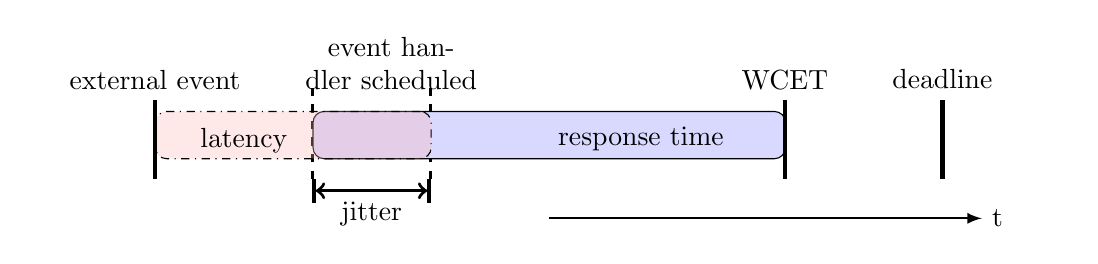
\begin{tikzpicture}
%\draw[gray, very thick, solid, >-<]  (0,1.5) -- (9,1.5) node at (4,1.5) [above] {relative deadline};
%\draw[black, very thick, ->]  (0,0) -- (10,0) node at (11,0) {time};
\draw[black, very thick, dashed] (2.0,0) -- (2.0,1.25) node at (3,1) [text width=3cm, above, align=center] {event handler scheduled};
\draw[black, very thick, dashed] (3.5,0) -- (3.5,1.25);

\node at (2.0,0.25)[rectangle, draw=black, fill=blue!15, rounded corners, minimum height = 0.6cm, minimum width = 6cm, anchor=south west] (resptime) {};

\begin{scope}[fill opacity=0.3]
\node at (0,0.25)[rectangle, draw=black, dashdotted, fill=red!30, rounded corners, minimum height = 0.6cm, minimum width = 3.50cm, anchor=south west] (latency) {};
%\node at (2.0,0.25)[rectangle, draw=black, postaction={pattern=north east lines}, minimum height = 0.6cm, minimum width = 1.5cm, anchor=south west] (overlap) {};
\end{scope}

\node [above left, inner sep=2pt] at (latency.south) {latency};
\node [above right, inner sep=3pt] at (resptime.south) {response time};

\draw[black, very thick, solid] (0,0) -- (0,1) node at (0,1) [text width=3cm, above, align=center] {external event};
\draw[black, very thick, solid] (8,0) -- (8,1) node at (8,1) [text width=3cm, above, align=center] {WCET};
\draw[black, ultra thick, solid] (10,0) -- (10,1) node at (10,1) [text width=3cm, above, align=center] {deadline};

\draw[black, very thick, solid, |<->|] (2.0,-0.15) -- (3.5,-0.15) node (jitter) at (2.75,-0.15) [below] {jitter};

%\node (latlabel) at (1,-1.0) {latency};
%\node (jitlabel) at (4,-1.0) {jitter};
%\node (rtlabel) at (8,-1.0) {response time};

\begin{scope}[>=latex]
	%\draw [thick, ->] (latlabel) to [bend right=45] (latency.center);
	%\draw [thick, ->] (rtlabel) to [bend left=45] (resptime.center);
    	%\draw [thick, ->] (jitlabel) to [bend left=45] (jitter.center);
	\draw[black, thick, ->] (5,-0.5) -- (10.5,-0.5) node [right] {t};
\end{scope}
\end{tikzpicture}
\end{center}
\ifreport
\caption{Real-time task interrupt latency and jitter}
\fi
\label{fig-latency-jitter}
\end{figure}

	\endgroup
    \pause{}
  \item {predictable response time} \pause{}
  \item {soft versus hard real-time}
  \end{itemize}
\end{frame}

%%%%%%%%%%%%%%%%%~~~SUB SECTION~~~%%%%%%%%%%%%%%%%%
\subsection{Virtualization}
\begin{frame}{Virtualization Technology}
  \begin{itemize}
  \item {hosting multiple virtual machines on one hardware platform}  \pause{}
  \item {software layer: VMM or Hypervisor}  \pause{}
   	\begingroup
	\tikzset{every picture/.style={scale=0.9}, every node/.style={scale=0.9}}
	\begin{figure}[!htb]
\begin{center}
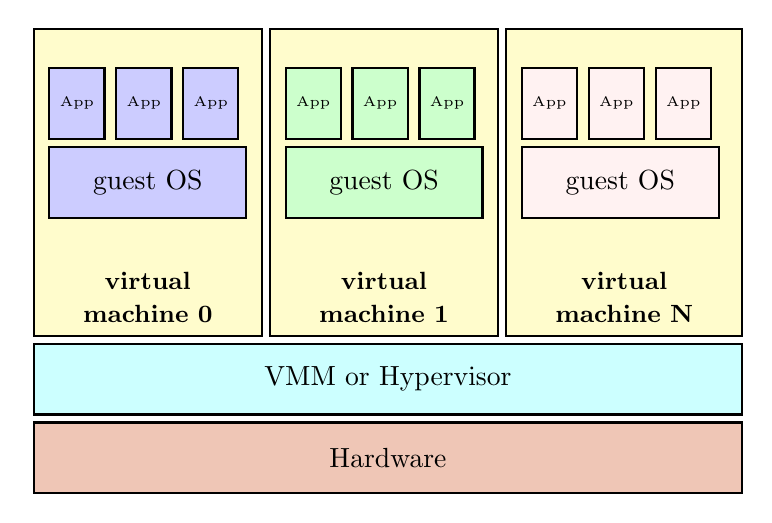
\begin{tikzpicture}

\node at (0,2) [rectangle, draw=black, thick, fill=yellow!20, minimum height = 3.9cm, minimum width = 2.9cm, anchor=south west] (vm0) {};
\node [above, inner sep=5pt, align=center, text width=2.7cm] at (vm0.south) {\textbf{\small{virtual\\ machine 0}}};

\node at (0.2,3.5) [rectangle, draw=black, thick, fill=blue!20, minimum height = 0.9cm, minimum width = 2.5cm, anchor=south west] (g0) {guest OS};
\node at (0.2,4.5) [rectangle, draw=black, thick, fill=blue!20, minimum height = 0.9cm, minimum width = 0.7cm, anchor=south west] (g0app0) {\tiny{App}};
\node at (0.2+0.85,4.5) [rectangle, draw=black, thick, fill=blue!20, minimum height = 0.9cm, minimum width = 0.7cm, anchor=south west] (g0app1) {\tiny{App}};
\node at (0.2+1.7,4.5) [rectangle, draw=black, thick, fill=blue!20, minimum height = 0.9cm, minimum width = 0.7cm, anchor=south west] (g0appn) {\tiny{App}};

\node at (3,2) [rectangle, draw=black, thick, fill=yellow!20, minimum height = 3.9cm, minimum width = 2.9cm, anchor=south west] (vm1) {};
\node [above, inner sep=5pt, align=center, text width=2.7cm] at (vm1.south) {\textbf{\small{virtual\\ machine 1}}};
\node at (3.2,3.5) [rectangle, draw=black, thick, fill=green!20, minimum height = 0.9cm, minimum width = 2.5cm, anchor=south west] (g1) {guest OS};
\node at (3.2,4.5) [rectangle, draw=black, thick, fill=green!20, minimum height = 0.9cm, minimum width = 0.7cm, anchor=south west] (g1app0) {\tiny{App}};
\node at (3.2+0.85,4.5) [rectangle, draw=black, thick, fill=green!20, minimum height = 0.9cm, minimum width = 0.7cm, anchor=south west] (g1app1) {\tiny{App}};
\node at (3.2+1.7,4.5) [rectangle, draw=black, thick, fill=green!20, minimum height = 0.9cm, minimum width = 0.7cm, anchor=south west] (g1appn) {\tiny{App}};

\node at (6,2) [rectangle, draw=black, thick, fill=yellow!20, minimum height = 3.9cm, minimum width = 3cm, anchor=south west] (vmn) {};
\node [above, inner sep=5pt, align=center, text width=2.7cm] at (vmn.south) {\textbf{\small{virtual\\ machine N}}};
\node at (6.2,3.5) [rectangle, draw=black, thick, fill=pink!20, minimum height = 0.9cm, minimum width = 2.5cm, anchor=south west] (gn) {guest OS};
\node at (6.2,4.5) [rectangle, draw=black, thick, fill=pink!20, minimum height = 0.9cm, minimum width = 0.7cm, anchor=south west] (gnapp0) {\tiny{App}};
\node at (6.2+0.85,4.5) [rectangle, draw=black, thick, fill=pink!20, minimum height = 0.9cm, minimum width = 0.7cm, anchor=south west] (gnapp1) {\tiny{App}};
\node at (6.2+1.7,4.5) [rectangle, draw=black, thick, fill=pink!20, minimum height = 0.9cm, minimum width = 0.7cm, anchor=south west] (gnappn) {\tiny{App}};

\node at (0,1) [rectangle, draw=black, thick, fill=Cyan!20, minimum height = 0.9cm, minimum width = 9cm, anchor=south west] (hyper) {VMM or Hypervisor};
\node at (0,0) [rectangle, draw=black, thick, fill=BrickRed!20, minimum height = 0.9cm, minimum width = 9cm, anchor=south west] (hard) {Hardware};


\end{tikzpicture}
\end{center}
\ifreport
\caption{Virtualization Technology}
\fi
\label{fig-virtualization}
\end{figure}

	\endgroup
    \pause{}
  \item {Types: type-I (bare-metal), type-II(hosted)} \pause{}
  \item {Benefits: software consolidation, cost reduction, security enhancement etc.}
  \end{itemize}
\end{frame}
\begin{frame}{Virtualization Techniques} {Classical Virtualization (trap-and-emulate)}
  \begin{itemize}
  %\item {requirements: Equivalence, Performance, Resource Control} \pause{}
  \item{sensitive instructions should be a subset of privileged instructions} \pause{}		
  %\item {guest traps whenever it tries to execute privileged instruction}  \pause{}
  	%\begingroup
	%\tikzset{every picture/.style={scale=0.8}, every node/.style={scale=0.8}}
	\begin{figure}[!htb]
\begin{center}
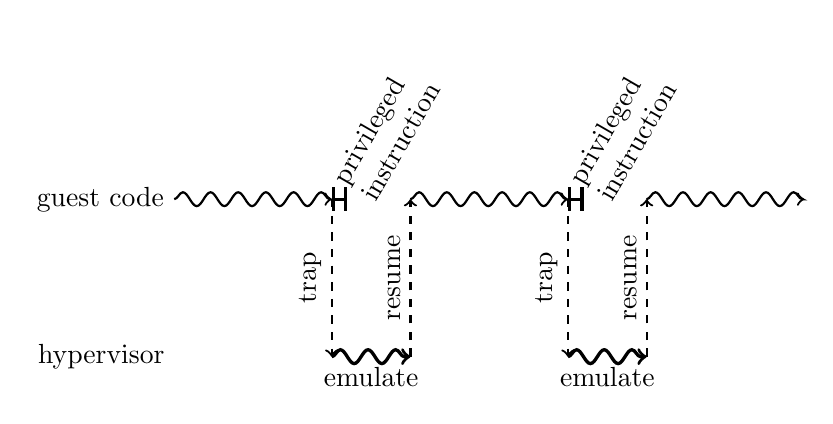
\begin{tikzpicture}


\draw[thick, decorate, decoration=snake, ->] (0, 2) -- (2, 2) node at (0,2) [left] {guest code};
\draw[very thick, |-|] (2, 2) -- (2.2, 2) node [above, right, rotate=60, text width=2cm]{privileged instruction};

\node at (0,0) [left] {hypervisor};
\draw[thick, dashed, ->] (2, 2) -- (2, 0) node [above, align=center,midway, rotate=90]{trap};
\draw[very thick, decorate, decoration=snake, ->] (2.0, 0) -- (3, 0) node [below,midway] {emulate};
\draw[thick, dashed, ->] (3, 0) -- (3, 2) node [above, align=center, midway, rotate=90] {resume};

\draw[thick, decorate, decoration=snake, ->] (3, 2) -- (5, 2);
\draw[very thick, |-|] (5, 2) -- (5.2, 2) node [above, right, rotate=60, text width=2cm]{privileged instruction};

\draw[thick, dashed, ->] (5, 2) -- (5, 0) node [above, align=center,midway, rotate=90]{trap};
\draw[very thick, decorate, decoration=snake, ->] (5, 0) -- (6, 0)  node [below,midway] {emulate};
\draw[thick, dashed, ->] (6, 0) -- (6, 2) node [above, align=center,midway, rotate=90]{resume};

\draw[thick, decorate, decoration=snake, ->] (6, 2) -- (8, 2);

\end{tikzpicture}
\end{center}
\ifreport
\caption{Faithful Virtualization (trap-and-emualte)}
\fi
\label{fig-virt-faithful}
\end{figure}

	%\endgroup
    \pause{}
  \item{Pros: supports unmodified guests (faithful virtualization)} \pause{}
  \item{Cons: requires hardware support}
  \end{itemize}
\end{frame}
\begin{frame}{Virtualization Techniques} {Software-based Virtualization}
  \begin{itemize}
  \item {Translation engine transforms all or sensitive instructions of guest code \pause{}}
  	%\begingroup
	%\tikzset{every picture/.style={scale=0.8}, every node/.style={scale=0.8}}
	\begin{figure}[!htb]
\begin{center}
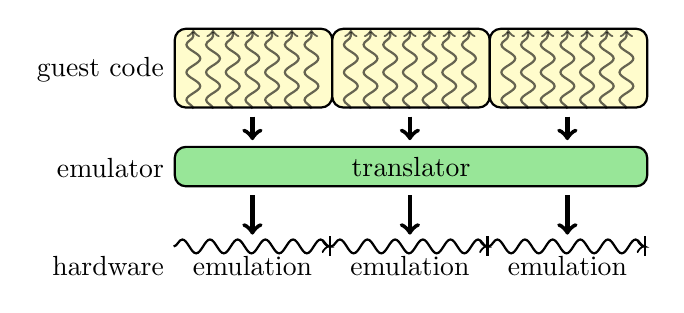
\begin{tikzpicture}

\node at (0,2.5) [left] {guest code};
\node at (0,2) [rectangle, draw=black, thick, rounded corners, fill=yellow!20,  minimum height = 1cm, minimum width = 2cm, anchor=south west] (b1) {};
\begin {scope} [opacity=0.6]
\draw[thick, decorate, decoration=snake, ->] (0.25, 2) -- (0.25, 3);
\draw[thick, decorate, decoration=snake, ->] (0.5, 2) -- (0.5, 3);
\draw[thick, decorate, decoration=snake, ->] (0.75, 2) -- (0.75, 3);
\draw[thick, decorate, decoration=snake, ->] (1, 2) -- (1, 3);
\draw[thick, decorate, decoration=snake, ->] (1.25, 2) -- (1.25, 3);
\draw[thick, decorate, decoration=snake, ->] (1.5, 2) -- (1.5, 3);
\draw[thick, decorate, decoration=snake, ->] (1.75, 2) -- (1.75, 3);
\end {scope}

\node at (2,2) [rectangle, draw=black, thick, rounded corners, fill=yellow!20, minimum height = 1cm, minimum width = 2cm, anchor=south west] (b2) {};
\begin {scope} [opacity=0.6]
\draw[thick, decorate, decoration=snake, ->] (2.25, 2) -- (2.25, 3);
\draw[thick, decorate, decoration=snake, ->] (2.5, 2) -- (2.5, 3);
\draw[thick, decorate, decoration=snake, ->] (2.75, 2) -- (2.75, 3);
\draw[thick, decorate, decoration=snake, ->] (3, 2) -- (3, 3);
\draw[thick, decorate, decoration=snake, ->] (3.25, 2) -- (3.25, 3);
\draw[thick, decorate, decoration=snake, ->] (3.5, 2) -- (3.5, 3);
\draw[thick, decorate, decoration=snake, ->] (3.75, 2) -- (3.75, 3);
\end {scope}

\node at (4,2) [rectangle, draw=black, thick, rounded corners, fill=yellow!20, minimum height = 1cm, minimum width = 2cm, anchor=south west] (b2) {};
\begin {scope} [opacity=0.6]
\draw[thick, decorate, decoration=snake, ->] (4.25, 2) -- (4.25, 3);
\draw[thick, decorate, decoration=snake, ->] (4.5, 2) -- (4.5, 3);
\draw[thick, decorate, decoration=snake, ->] (4.75, 2) -- (4.75, 3);
\draw[thick, decorate, decoration=snake, ->] (5, 2) -- (5, 3);
\draw[thick, decorate, decoration=snake, ->] (5.25, 2) -- (5.25, 3);
\draw[thick, decorate, decoration=snake, ->] (5.5, 2) -- (5.5, 3);
\draw[thick, decorate, decoration=snake, ->] (5.75, 2) -- (5.75, 3);
\end {scope}

\draw[ultra thick, ->] (1, 1.9) -- (1, 1.6);
\draw[ultra thick, ->] (3, 1.9) -- (3, 1.6);
\draw[ultra thick, ->] (5, 1.9) -- (5, 1.6);
\draw[ultra thick, ->] (1, 0.9) -- (1, 0.4);
\draw[ultra thick, ->] (3, 0.9) -- (3, 0.4);
\draw[ultra thick, ->] (5, 0.9) -- (5, 0.4);

\node at (0,1) [rectangle, draw=black, thick, rounded corners,  fill=LimeGreen!50, minimum height = 0.5cm, minimum width = 6cm, anchor=south west] (tr) {translator};
\node at (0,1.25) [left] {emulator};

\node at (0,0) [left] {hardware};
\draw[thick, decorate, decoration=snake, ->|] (0, 0.25) -- (2, 0.25)  node [below, align=center, midway, text width=2cm] {emulation};
\draw[thick, decorate, decoration=snake, ->|] (2, 0.25) -- (4, 0.25)  node [below, align=center, midway, text width=2cm] {emulation};
\draw[thick, decorate, decoration=snake, ->|] (4, 0.25) -- (6, 0.25)  node [below, align=center, midway, text width=2cm] {emulation};

\end{tikzpicture}
\end{center}
\ifreport
\caption{Software-based Virtualization}
\fi
\label{fig-virt-software}
\end{figure}

	%\endgroup
	\pause{}
  \item{Examples: QEMU, VMware Workstation, VirtualBox}  \pause{}
  \item{Pros: guest and hardware ISA can be different, unmodified guest} \pause{}
  \item{Cons: emulation overhead}

  \end{itemize}
\end{frame}
\begin{frame}{Virtualization Techniques} {Paravirtualization}
  \begin{itemize}
  \item {Sensitive instructions are replaced with hypercalls \pause{}}  
  	%\begingroup
	%\tikzset{every picture/.style={scale=0.8}, every node/.style={scale=0.8}}	
	\begin{figure}[!htb]
\begin{center}
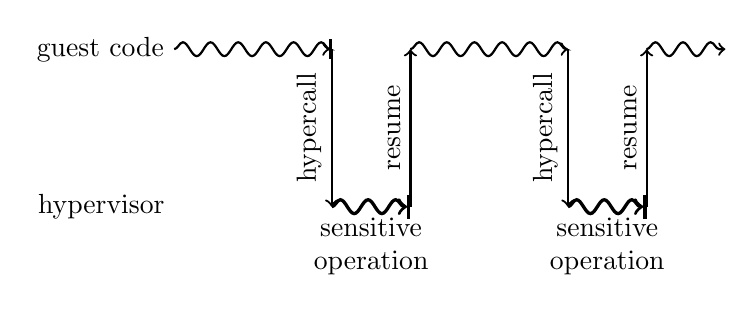
\begin{tikzpicture}


\draw[thick, decorate, decoration=snake, ->|] (0, 2) -- (2, 2) node at (0,2) [left] {guest code};
%\draw[thick, |-|] (2, 2) -- (2.3, 2) ; node [right, rotate=90, text width=2cm]{sensitive instruction};

\node at (0,0) [left] {hypervisor};
\draw[thick, ->] (2, 2) -- (2, 0) node [above, align=center,midway, rotate=90]{hypercall};
\draw[very thick, decorate, decoration=snake, ->|] (2.0, 0) -- (3, 0)   node [below, align=center, midway, text width=2cm] {sensitive operation};
\draw[thick, ->] (3, 0) -- (3, 2) node [above, align=center, midway, rotate=90] {resume};

\draw[thick, decorate, decoration=snake, ->] (3, 2) -- (5, 2);
%\draw[thick, |-|] (5, 2) -- (5.3, 2) node [right, rotate=90, text width=2cm]{sensitive operation};

\draw[thick, ->] (5, 2) -- (5, 0) node [above, align=center,midway, rotate=90]{hypercall};
\draw[very thick, decorate, decoration=snake, ->|] (5, 0) -- (6, 0)  node [below, align=center, midway, text width=2cm] {sensitive operation};
\draw[thick, ->] (6, 0) -- (6, 2) node [above, align=center,midway, rotate=90]{resume};

\draw[thick, decorate, decoration=snake, ->] (6, 2) -- (7, 2);

\end{tikzpicture}
\end{center}
\ifreport
\caption{Paravirtualization}
\fi
\label{fig-virt-para}
\end{figure}

	%\endgroup
	\pause{}
  \item{Examples: Xen} \pause{}
  \item{Pros: near native performance} \pause{}
  \item{Cons: guest has to be modified}

  \end{itemize}
\end{frame}

\begin{frame}{Virtualization of Real-time Applications}
  \begin{itemize}
 %%	 \item {traditional virtualization solutions does not address real-time issues:} \pause{}
 %%	 		\begin{itemize}
 %%				\item{deterministic response times} \pause{}
 %%			\item{complexity, footprint} \pause{}
 %%		\end{itemize}
  \item {real-time virtualization solutions also exist} \pause{}
 		\begin{itemize}
			\item{industry specific: Xtratum for safety-critical applications} \pause{}
			\item{custom designed: WindRiver hypervisor for VxWorks} \pause{}
			\item{real-time extensions: \pause{}RT-Xen (Xen with real-time framework), \pause{}KVM with PREEMPT\_RT patch} \pause{}
			\item{microkernel based: OKL4 Microvisor} \pause{}
			\item{resource partitioning: Quest-V}
		\end{itemize}  
  \end{itemize}
\end{frame}

%% \begin{frame}{Virtual Machines on Multicore Processors}
%%   \begin{itemize}
%%   \item {real-time app. on single core processors} \pause{}
%%   \item {multicore platforms has become a norm} \pause{}
%%   \item {designers have embraced multicore} \pause{}
%%   \item {heterogeneous and manycore processor platforms} \pause{}
%%   \item {user demands: complex software stacks} \pause{}
%%   \item {require timing guarantees, not so much computing resources} \pause{}
%%   \item {allows consolidation} \pause{}
%%   \item {dedicated CPU cores} 
%%  \end{itemize}
%% \end{frame}

%%%%%%%%%%%%%%%%%~~~SUB SECTION~~~%%%%%%%%%%%%%%%%%
\subsection{Hardware-assisted Virtualization on x86}
\begin{frame}{Hardware-assisted Virtualization on x86} {modes of operation}
		\begin{table}[H]
		\centering
		\begin{longtable}{|r|c|c|} 
		\hline
			\textbf{CPU operation mode}	&	{\textbf{VMX non-root}} 	&	{\textbf{VMX root}} \\ \hline \hline
			Instruction set		&	privileged instructions 		&  new instruction added \\
				                &	are restricted (e.g. out	&  to manage VMs \\ 
				                &	instruction cause trap to   & (e.g. VMLAUNCH,  \\ 
				                &	VMX root mode)              & VMREAD, VMWRITE) \\ \hline
			Software 			&	OS (Kernel and User)	&	Hypervisor \\ \hline
		\end{longtable}
		\end{table}

		\begin{itemize}
			\item {VMX transitions: vmexit, vmentry}
		\end{itemize}
\end{frame}

\begin{frame}{Hardware-assisted Virtualization on x86} {VMCS}
 	\begingroup
	\tikzset{every picture/.style={scale=0.8}, every node/.style={scale=0.8}}	
	\begin{figure}[!htb]
\begin{center}
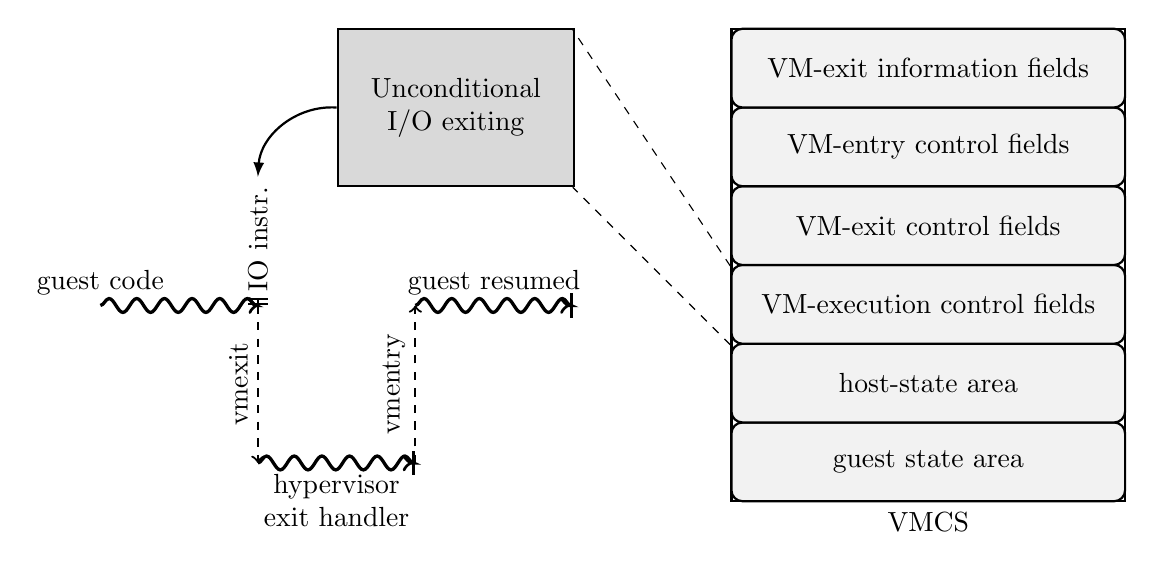
\begin{tikzpicture}

%\draw[step=0.5cm, gray, very thin] (0,0) grid (9,9)


\draw[very thick, decorate, decoration=snake, ->] (0, 2.5) -- (2, 2.5) node at (0,2.5) [above] {guest code};
\draw[thick, |-|] (2, 2.5) -- (2, 2.6) node at (2, 2.6)[right, midway, rotate=90] (ioinst) {IO instr.};

\draw[very thick, decorate, decoration=snake, ->|] (2, 0.5) -- (4, 0.5) node [below, midway, align=center] {hypervisor\\ exit handler};
\draw[very thick, decorate, decoration=snake, ->|] (4, 2.5) -- (6, 2.5) node [above, align=center, midway] {guest resumed};

\draw[thick, dashed, ->] (2, 2.5) -- (2, 0.5) node [above, align=center,midway, rotate=90] {vmexit};
\draw[thick, dashed, ->] (4, 0.5) -- (4, 2.5) node [above, align=center,midway, rotate=90] {vmentry};


\node at (3,4) [rectangle, draw=black, thick, fill=black!15, minimum height = 2cm, minimum width = 3cm, anchor=south west, align=center] (exitcontrol) 
                        {Unconditional\\ I/O exiting} ;


\node at (8,0) [rectangle, draw=black, thick, fill=white, minimum height = 6cm, minimum width = 5cm, anchor=south west] (vmcs) {} ;
\node [below, align=center] at (vmcs.south) {VMCS};
%\node[below right, inner sep=5pt, text width=2cm] at (rtguest.north west) {PREEMPT\_RT\\ Linux\\ (rt-guest)};


\node at (8,0) [rectangle, draw=black, thick, rounded corners, fill=black!5, minimum height = 1cm, minimum width = 5cm, anchor=south west] (gstate) {guest state area};
\node at (8,1) [rectangle, draw=black, thick, rounded corners, fill=black!5, minimum height = 1cm, minimum width = 5cm, anchor=south west] (gstate) {host-state area};
\node at (8,2) [rectangle, draw=black, thick, rounded corners, fill=black!5, minimum height = 1cm, minimum width = 5cm, anchor=south west] (gstate) {VM-execution control fields};
\node at (8,3) [rectangle, draw=black, thick, rounded corners, fill=black!5, minimum height = 1cm, minimum width = 5cm, anchor=south west] (gstate) {VM-exit control fields};
\node at (8,4) [rectangle, draw=black, thick, rounded corners, fill=black!5, minimum height = 1cm, minimum width = 5cm, anchor=south west] (gstate) {VM-entry control fields};
\node at (8,5) [rectangle, draw=black, thick, rounded corners, fill=black!5, minimum height = 1cm, minimum width = 5cm, anchor=south west] (gstate) {VM-exit information fields};

\draw [dashed] (8,2) -- (6,4); 
\draw [dashed] (8,3) -- (6,6); 

\begin{scope}[>=latex]
	\draw [thick, ->] (exitcontrol.west) to [bend right=45] (ioinst.east);
\end{scope}

\end{tikzpicture}
\end{center}
\ifreport
\caption{VMCS data structure with an example of using VMCS fields to control guest execution behavior}
\fi
\label{fig-vmcs-ds}
\end{figure}

	\endgroup
\end{frame}

\begin{frame}{Features for Efficient Virtualization} {MMU Virtualization}
 	\begingroup
	\tikzset{every picture/.style={scale=0.55}, every node/.style={scale=0.55}}	
	\begin{figure}[!htb]
\begin{center}
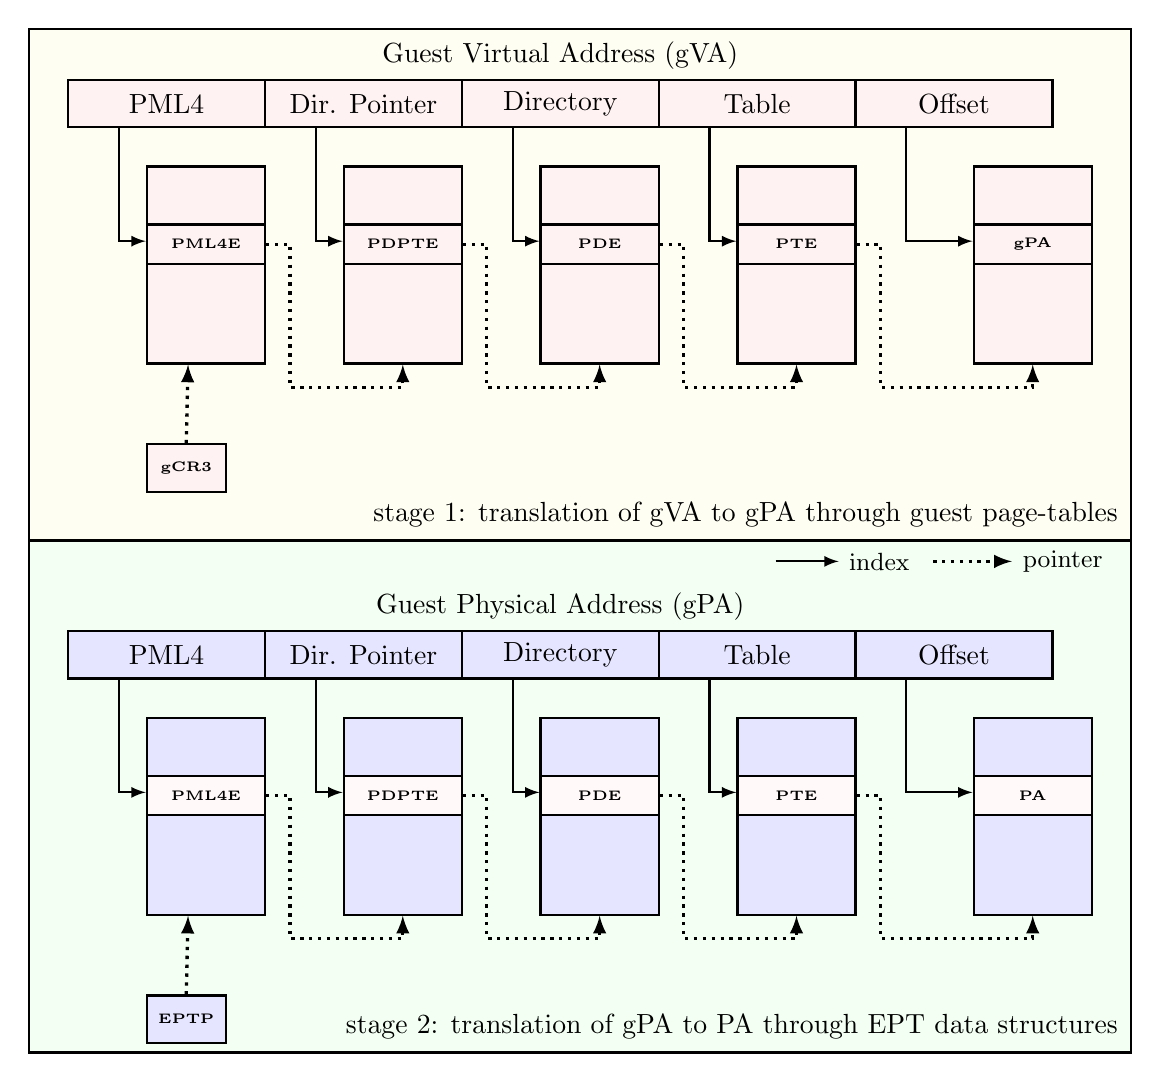
\begin{tikzpicture}

\node at (-0.5,-5-0.25) [rectangle, draw=black, thick, fill=yellow!5, minimum height = 6.5cm, minimum width = 14cm, anchor=south west] (stage1) {};
\node [above left, inner sep=5pt] at (stage1.south east) {\textbf\small{{stage 1: translation of gVA to gPA through guest page-tables}}};

\node at (0,0) [rectangle, draw=black, thick, fill=pink!20, minimum height = 0.6cm, minimum width = 2.5cm, anchor=south west] (gpml4) {PML4};
\node at (0+2.5,0) [rectangle, draw=black, thick, fill=pink!20, minimum height = 0.6cm, minimum width = 2.5cm, anchor=south west] (gdirptr) {Dir. Pointer};
\node at (0+2.5+2.5,0) [rectangle, draw=black, thick, fill=pink!20, minimum height = 0.6cm, minimum width = 2.5cm, anchor=south west] (gdir) {Directory};
\node [above, align=center] at (gdir.north) {\textbf\small{{Guest Virtual Address (gVA)}}};
\node at (0+2.5+2.5+2.5,0) [rectangle, draw=black, thick, fill=pink!20, minimum height = 0.6cm, minimum width = 2.5cm, anchor=south west] (gtbl) {Table};
\node at (0+2.5+2.5+2.5+2.5,0) [rectangle, draw=black, thick, fill=pink!20, minimum height = 0.6cm, minimum width = 2.5cm, anchor=south west] (goff) {Offset};


\node at (1.0,-3) [rectangle, draw=black, thick, fill=pink!20, minimum height = 2.5cm, minimum width = 1.5cm, anchor=south west] (gpgpml4) {};
\node [rectangle, draw=black, thick, fill=pink!20, minimum height = 0.5cm, minimum width = 1.5cm, anchor=south west] at (gpgpml4.west) (gpgpml4e) 
				{\tiny\textbf{{PML4E}}};

\node at (1.0,-4)  [rectangle, draw=black, thick, fill=pink!20, minimum height = 0.6cm, minimum width = 1.0cm, anchor=north west] (gcr3) 
				{\tiny\textbf{{gCR3}}};

\node at (3.5,-3) [rectangle, draw=black, thick, fill=pink!20, minimum height = 2.5cm, minimum width = 1.5cm, anchor=south west] (gpgdirptr) {};
\node [rectangle, draw=black, thick, fill=pink!20, minimum height = 0.5cm, minimum width = 1.5cm, anchor=south west] at (gpgdirptr.west) 
			    (gpgdirptre) {\tiny\textbf{{PDPTE}}};
\node at (6,-3) [rectangle, draw=black, thick, fill=pink!20, minimum height = 2.5cm, minimum width = 1.5cm, anchor=south west] (gpgdir) {};
\node [rectangle, draw=black, thick, fill=pink!20, minimum height = 0.5cm, minimum width = 1.5cm, anchor=south west] at (gpgdir.west) 
                (gpgdire) {\tiny\textbf{{PDE}}};
\node at (8.5,-3) [rectangle, draw=black, thick, fill=pink!20, minimum height = 2.5cm, minimum width = 1.5cm, anchor=south west] (gpgtbl) {};
\node [rectangle, draw=black, thick, fill=pink!20, minimum height = 0.5cm, minimum width = 1.5cm, anchor=south west] at (gpgtbl.west) 
                (gpgtble) {\tiny\textbf{{PTE}}};
\node at (11.5,-3) [rectangle, draw=black, thick, fill=pink!20, minimum height = 2.5cm, minimum width = 1.5cm, anchor=south west] (gpgoff) {};
\node [rectangle, draw=black, thick, fill=pink!20, minimum height = 0.5cm, minimum width = 1.5cm, anchor=south west] at (gpgoff.west) 
                {\tiny\textbf{{gPA}}};


\begin{scope}[>=latex]	
	\draw [thick, ->] ([xshift=-4ex]gpml4.south) |- ([yshift=2ex]gpgpml4.west);
	\draw [thick, ->] ([xshift=-4ex]gdirptr.south) |- ([yshift=2ex]gpgdirptr.west);
	\draw [thick, ->] ([xshift=-4ex]gdir.south) |- ([yshift=2ex]gpgdir.west);
	\draw [thick, ->] ([xshift=-4ex]gtbl.south) |- ([yshift=2ex]gpgtbl.west);
	\draw [thick, ->] ([xshift=-4ex]goff.south) |- ([yshift=2ex]gpgoff.west);

	%\draw [thick, dotted, ->] ([yshift=-1ex]gpgpml4e.south) to [bend right=75] (gpgdirptr.south);

	\draw [very thick, dotted, ->] (gcr3.north) -- ([xshift=-1.5ex]gpgpml4.south);
	\draw [very thick, dotted, ->] (gpgpml4e.east) -| ([xshift=2ex]gpgpml4e.east) -- ([xshift=2ex, yshift=-12ex]gpgpml4e.east) -| (gpgdirptr.south);
	\draw [very thick, dotted, ->] (gpgdirptre.east) -| ([xshift=2ex]gpgdirptre.east) -- ([xshift=2ex, yshift=-12ex]gpgdirptre.east) -| (gpgdir.south);
	\draw [very thick, dotted, ->] (gpgdire.east) -| ([xshift=2ex]gpgdire.east) -- ([xshift=2ex, yshift=-12ex]gpgdire.east) -| (gpgtbl.south);
	\draw [very thick, dotted, ->] (gpgtble.east) -| ([xshift=2ex]gpgtble.east) -- ([xshift=2ex, yshift=-12ex]gpgtble.east) -| (gpgoff.south);	

\end{scope}

\node at (-0.5,-5-7+0.25) [rectangle, draw=black, thick, fill=green!5, minimum height = 6.5cm, minimum width = 14cm, anchor=south west] (stage2) {};
\node [above left, inner sep=5pt] at (stage2.south east) {\textbf\small{{stage 2: translation of gPA to PA through EPT data structures}}};

\node at (0,0-7) [rectangle, draw=black, thick, fill=blue!10, minimum height = 0.6cm, minimum width = 2.5cm, anchor=south west] (gpml4) {PML4};
\node at (0+2.5,0-7) [rectangle, draw=black, thick, fill=blue!10, minimum height = 0.6cm, minimum width = 2.5cm, anchor=south west] (gdirptr) {Dir. Pointer};
\node at (0+2.5+2.5,0-7) [rectangle, draw=black, thick, fill=blue!10, minimum height = 0.6cm, minimum width = 2.5cm, anchor=south west] (gdir) {Directory};
\node [above, align=center] at (gdir.north) {\textbf\small{{Guest Physical Address (gPA)}}};
\node at (0+2.5+2.5+2.5,0-7) [rectangle, draw=black, thick, fill=blue!10, minimum height = 0.6cm, minimum width = 2.5cm, anchor=south west] (gtbl) {Table};
\node at (0+2.5+2.5+2.5+2.5,0-7) [rectangle, draw=black, thick, fill=blue!10, minimum height = 0.6cm, minimum width = 2.5cm, anchor=south west] (goff) {Offset};


\node at (1.0,-3-7) [rectangle, draw=black, thick, fill=blue!10, minimum height = 2.5cm, minimum width = 1.5cm, anchor=south west] (gpgpml4) {};
\node [rectangle, draw=black, thick, fill=pink!10, minimum height = 0.5cm, minimum width = 1.5cm, anchor=south west] at (gpgpml4.west) (gpgpml4e) 
				{\tiny\textbf{{PML4E}}};

\node at (1.0,-4-7)  [rectangle, draw=black, thick, fill=blue!10, minimum height = 0.6cm, minimum width = 1.0cm, anchor=north west] (eptp) 
				{\tiny\textbf{{EPTP}}};

\node at (3.5,-3-7) [rectangle, draw=black, thick, fill=blue!10, minimum height = 2.5cm, minimum width = 1.5cm, anchor=south west] (gpgdirptr) {};
\node [rectangle, draw=black, thick, fill=pink!10, minimum height = 0.5cm, minimum width = 1.5cm, anchor=south west] at (gpgdirptr.west) 
			    (gpgdirptre) {\tiny\textbf{{PDPTE}}};
\node at (6,-3-7) [rectangle, draw=black, thick, fill=blue!10, minimum height = 2.5cm, minimum width = 1.5cm, anchor=south west] (gpgdir) {};
\node [rectangle, draw=black, thick, fill=pink!10, minimum height = 0.5cm, minimum width = 1.5cm, anchor=south west] at (gpgdir.west) 
                (gpgdire) {\tiny\textbf{{PDE}}};
\node at (8.5,-3-7) [rectangle, draw=black, thick, fill=blue!10, minimum height = 2.5cm, minimum width = 1.5cm, anchor=south west] (gpgtbl) {};
\node [rectangle, draw=black, thick, fill=pink!10, minimum height = 0.5cm, minimum width = 1.5cm, anchor=south west] at (gpgtbl.west) 
                (gpgtble) {\tiny\textbf{{PTE}}};
\node at (11.5,-3-7) [rectangle, draw=black, thick, fill=blue!10, minimum height = 2.5cm, minimum width = 1.5cm, anchor=south west] (gpgoff) {};
\node [rectangle, draw=black, thick, fill=pink!10, minimum height = 0.5cm, minimum width = 1.5cm, anchor=south west] at (gpgoff.west) 
                {\tiny\textbf{{PA}}};

\begin{scope}[>=latex]	
	\draw [thick, ->] ([xshift=-4ex]gpml4.south) |- ([yshift=2ex]gpgpml4.west);
	\draw [thick, ->] ([xshift=-4ex]gdirptr.south) |- ([yshift=2ex]gpgdirptr.west);
	\draw [thick, ->] ([xshift=-4ex]gdir.south) |- ([yshift=2ex]gpgdir.west);
	\draw [thick, ->] ([xshift=-4ex]gtbl.south) |- ([yshift=2ex]gpgtbl.west);
	\draw [thick, ->] ([xshift=-4ex]goff.south) |- ([yshift=2ex]gpgoff.west);

	\draw [very thick, dotted, ->] (eptp.north) -- ([xshift=-1.5ex]gpgpml4.south);
	\draw [very thick, dotted, ->] (gpgpml4e.east) -| ([xshift=2ex]gpgpml4e.east) -- ([xshift=2ex, yshift=-12ex]gpgpml4e.east) -| (gpgdirptr.south);
	\draw [very thick, dotted, ->] (gpgdirptre.east) -| ([xshift=2ex]gpgdirptre.east) -- ([xshift=2ex, yshift=-12ex]gpgdirptre.east) -| (gpgdir.south);
	\draw [very thick, dotted, ->] (gpgdire.east) -| ([xshift=2ex]gpgdire.east) -- ([xshift=2ex, yshift=-12ex]gpgdire.east) -| (gpgtbl.south);
	\draw [very thick, dotted, ->] (gpgtble.east) -| ([xshift=2ex]gpgtble.east) -- ([xshift=2ex, yshift=-12ex]gpgtble.east) -| (gpgoff.south);	

	\draw [very thick, dotted, ->] (11,-5.5) -- (12, -5.5) node [right] {\small{pointer}};
	\draw [thick, ->] (9,-5.5) -- (9.8, -5.5) node [right] {\small{index}};
\end{scope}

\end{tikzpicture}
\end{center}
\ifreport
\caption{MMU Virtualization}
\fi
\label{fig-vmmu}
\end{figure}

	\endgroup
\end{frame}

\begin{frame}{Features for Efficient Virtualization} {TLB Partitioning}
	\begin{itemize}
		\item {VPID (Virtual Process Identifiers) allow hypervisor to separate address translations}
	\end{itemize}
	\begin{table}[!h]
	\centering
	\begin{tabular}{|c||c|c|c|}  
	\hline
		\textbf{TLB Entry}	&	\textbf{VPID}	&	\textbf{Tag} &	\textbf{Data}\\ \hline \hline
		Guest			&	x $(x > 0)$		&		gVA 	 & 	gPA			 \\ \hline
		Hypervisor		&	0				&		VA 		 &  PA			 \\ \hline
	\end{tabular}
	\label{vpid-entries}
	\end{table}
\end{frame}

\begin{frame}{Features for Efficient Virtualization} {APIC Virtualization}
  %\begin{itemize}
  %\item {EPT and VPIDs}
  %\end{itemize}
 	\begingroup
	\tikzset{every picture/.style={scale=0.7}, every node/.style={scale=0.7}}	
	\begin{figure}[!htb]
\begin{center}
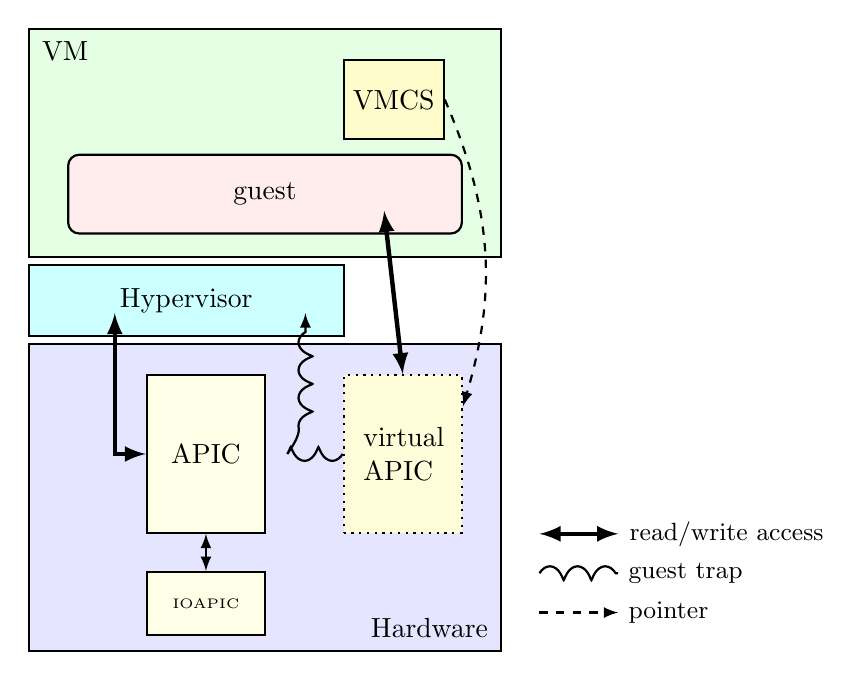
\begin{tikzpicture}

\node at (0,5) [rectangle, draw=black, thick, fill=green!10, minimum height = 2.9cm, minimum width = 6cm, anchor=south west] (vm) {};
\node [below right, inner sep=5pt] at (vm.north west) {VM};

\node at (0.5,5.3) [rectangle, rounded corners, draw=black, thick, fill=pink!30, minimum height = 1cm, minimum width = 5cm, anchor=south west] (g) {guest};
\node at (4.0,6.5) [rectangle, draw=black, thick, fill=yellow!20, minimum height = 1cm, minimum width = 0.5cm, anchor=south west] (vmcs) {VMCS};

\node at (0,4) [rectangle, draw=black, thick, fill=Cyan!20, minimum height = 0.9cm, minimum width = 4cm, anchor=south west] (hyper) {Hypervisor};

\node at (0,0) [rectangle, draw=black, thick, fill=blue!10, minimum height = 3.9cm, minimum width = 6cm, anchor=south west] (hard) {};
\node [above left, inner sep=5pt] at (hard.south east) {Hardware};

\node at (1.5,1.5) [rectangle, draw=black, thick, fill=yellow!10, minimum height = 2cm, minimum width = 1.5cm, anchor=south west] (apic) {APIC};
\node at (1.5,0.2) [rectangle, draw=black, thick, fill=yellow!10, minimum height = 0.8cm, minimum width = 1.5cm, anchor=south west] (ioapic) {\tiny{IOAPIC}};

\node at (4,1.5) [dotted, rectangle, draw=black, thick, fill=yellow!15, minimum height = 2cm, minimum width = 1.5cm, anchor=south west, text width=1cm] (vapic) {virtual APIC};

\begin{scope}[>=latex]	
	\draw [ultra thick, <->] (apic.west) -| ([xshift=-6ex, yshift=2ex]hyper.south) ;
	\draw [ultra thick, <->] ([xshift=10ex, yshift=2ex]g.south) -- (vapic.north) ;
	\draw [thick,  decorate, decoration=coil, ->] (vapic.west) -| ([xshift=10ex, yshift=2ex]hyper.south) ;
	\draw [thick, dashed, ->] (vmcs.east) to [bend left=20] ([yshift=4ex]vapic.east) ;
	\draw [thick, <->] (apic.south) -- (ioapic.north) ;

	\draw [ultra thick, <->] (6.5,1.5) -- (7.5,1.5) node [right] {\small{read/write access}};
	\draw [thick, decorate, decoration=coil] (6.5,1) -- (7.5,1) node [right] {\small{guest trap}};
	\draw [thick, dashed, ->] (6.5,0.5) -- (7.5,0.5) node [right] {\small{pointer}};
\end{scope}



\end{tikzpicture}
\end{center}
\ifreport
\caption{APIC Virtualization}
\fi
\label{fig-vapic}
\end{figure}

	\endgroup
\end{frame}

\begin{frame}{Features for Efficient Virtualization} {Direct Interrupt Injection}
  \begin{itemize}
  	\item {supports Posted Interrupts (PI)}
  	\item {Hypervisor can inject guest interrupts without exit}
  \end{itemize}

 	\begingroup
	\tikzset{every picture/.style={scale=0.7}, every node/.style={scale=0.7}}	
	\begin{figure}[!htb]
\begin{center}
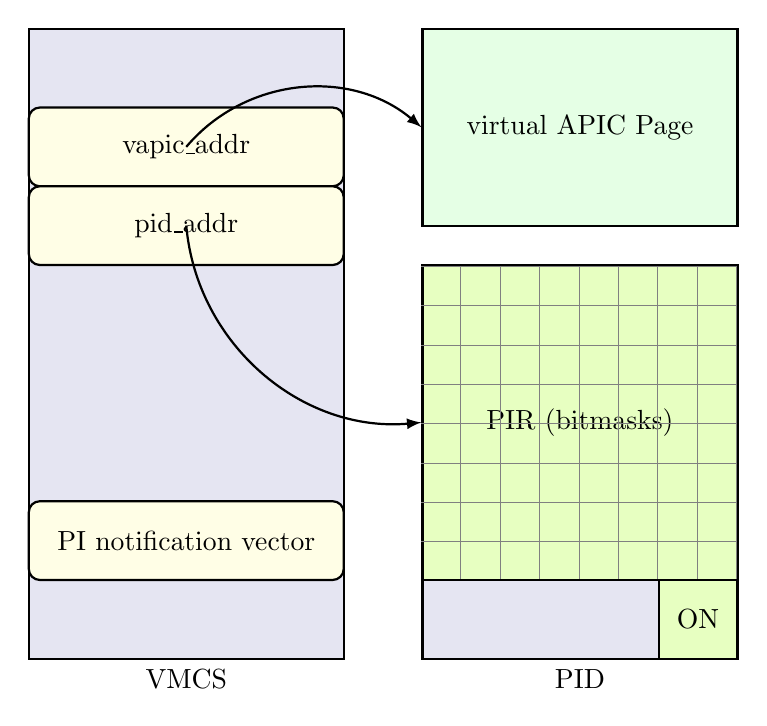
\begin{tikzpicture}


%%\draw[step=0.5cm, gray, very thin] (0,0) grid (9,9);

\node at (0,0) [rectangle, draw=black, thick, fill=NavyBlue!10, minimum height = 8cm, minimum width = 4cm, anchor=south west] (vmcs) {} ;
\node [below, align=center] at (vmcs.south) {VMCS};

\node at (0,6) [rectangle, draw=black, thick, fill=yellow!10, rounded corners, minimum height = 1cm, minimum width = 4cm, anchor=south west] (apicaddr)  {vapic\_addr};
\node at (0,5) [rectangle, draw=black, thick, fill=yellow!10, rounded corners, minimum height = 1cm, minimum width = 4cm, anchor=south west] (pidaddr)  {pid\_addr};

\node at (0,1) [rectangle, draw=black, thick, fill=yellow!10, rounded corners, minimum height = 1cm, minimum width = 4cm, anchor=south west] (pinv)  {PI notification vector};

\node at (5,1) [rectangle, draw=black, thick, fill=GreenYellow!30, minimum height = 4cm, minimum width = 4cm, anchor=south west] (pir) {PIR (bitmasks)};
\begin{scope}[fill opacity=0.9]
	\draw[xstep=0.5cm, ystep=0.5, gray, very thin] (5,1) grid (9,5);
\end{scope}

\node at (5,0) [rectangle, draw=black, thick, fill=NavyBlue!10, minimum height = 1cm, minimum width = 4cm, anchor=south west] (rsrvd) {};
\node at (8,0) [rectangle, draw=black, thick, fill=GreenYellow!30, minimum height = 1cm, minimum width = 1cm, anchor=south west] (on) {ON};
\node [below, align=center] at (rsrvd.south) {PID};

\node at (5,5.5) [rectangle, draw=black, thick, fill=green!10, minimum height = 2.5cm, minimum width = 4cm, anchor=south west] (vapic) {virtual APIC Page};


\begin{scope}[>=latex]
	\draw [thick, ->] (apicaddr.center) to [bend left=45] (vapic.west);
	\draw [thick, ->] (pidaddr.center) to [bend right=45] (pir.west);
\end{scope}


\end{tikzpicture}
\end{center}
\ifreport
\caption{Key data structures for Posted Interrupt processing. Virtual APIC page is used by VT-x to virtualize interrupt controller memory accesses. 
PINV is the interrupt vector number that uses PID data structure for delivery without exit.
PID consists of an ON bit and PIR bitmasks. Host marks PIR bit corresponding to interrupt vector and sets the ON bit
to deliver interrupt directly to the guest.}
\fi
\label{fig-pi-ds}
\end{figure}

	\endgroup
\end{frame}

\begin{frame}{Features for Efficient Virtualization} {Comparison of Interrupt Delivery}
  %\begin{itemize}
  %\item {DII}
  %\end{itemize}
 	\begingroup
	\tikzset{every picture/.style={scale=0.8}, every node/.style={scale=0.8}}	
	\begin{figure}[!htb]
\begin{center}
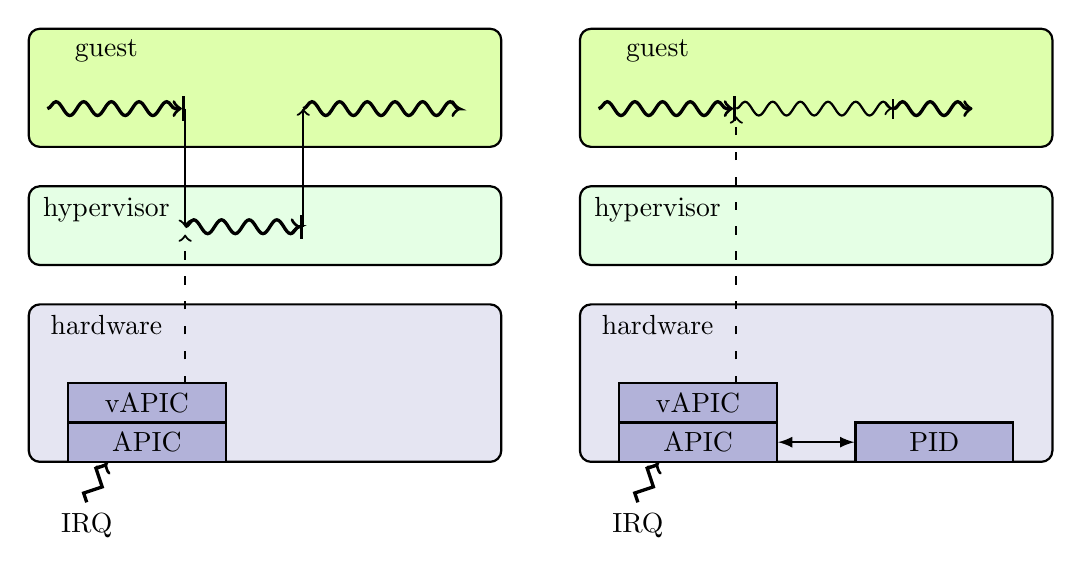
\begin{tikzpicture}


%\draw[step=0.5cm, gray, very thin] (0,0) grid (10,10);

\node at (0,0) [rectangle, draw=black, thick, rounded corners, fill=NavyBlue!10, minimum height = 2cm, minimum width = 6cm, anchor=south west] (hardware1) {} ;
\node at (1,2) [below] {hardware};
\node at (7,0) [rectangle, draw=black, thick, rounded corners, fill=NavyBlue!10, minimum height = 2cm, minimum width = 6cm, anchor=south west] (hardware2) {} ;
\node at (8,2) [below] {hardware};

\node at (0.5,0) [rectangle, draw=black, thick, fill=NavyBlue!30, minimum height = 0.5cm, minimum width = 2cm, anchor=south west] (apic1) {APIC};
\node at (7.5,0) [rectangle, draw=black, thick, fill=NavyBlue!30, minimum height = 0.5cm, minimum width = 2cm, anchor=south west] (apic2) {APIC};

\node at (0.5,0.5) [rectangle, draw=black, thick, fill=NavyBlue!30, minimum height = 0.5cm, minimum width = 2cm, anchor=south west] (vapic1) {vAPIC};
\node at (7.5,0.5) [rectangle, draw=black, thick, fill=NavyBlue!30, minimum height = 0.5cm, minimum width = 2cm, anchor=south west] (vapic2) {vAPIC};

\node at (10.5,0) [rectangle, draw=black, thick, fill=NavyBlue!30, minimum height = 0.5cm, minimum width = 2cm, anchor=south west] (pid2) {PID};

\node at (0,2.5) [rectangle, draw=black, thick, rounded corners, fill=green!10, minimum height = 1cm, minimum width = 6cm, anchor=south west] (phidias1) {} ;
\node at (1,3.5) [below] {hypervisor};
\node at (7,2.5) [rectangle, draw=black, thick, rounded corners, fill=green!10, minimum height = 1cm, minimum width = 6cm, anchor=south west] (phidias2) {} ;
\node at (8,3.5) [below] {hypervisor};

\node at (0,4) [rectangle, draw=black, thick, rounded corners, fill=GreenYellow!40, minimum height = 1.5cm, minimum width = 6cm, anchor=south west] (guest1) {} ;
\node at (1,5.5) [below] {guest};
\node at (7,4) [rectangle, draw=black, thick, rounded corners, fill=GreenYellow!40, minimum height = 1.5cm, minimum width = 6cm, anchor=south west] (guest2) {} ;
\node at (8,5.5) [below] {guest};

\draw[very thick, decorate, decoration=snake, ->|] (0.25, 4.5) -- (2, 4.5);
\draw[thick, ->] (2, 4.5) -- (2, 3);
\draw[very thick, decorate, decoration=snake, ->|] (2.0, 3) -- (3.5, 3);
\draw[thick, ->] (3.5, 3) -- (3.5, 4.5);
\draw[very thick, decorate, decoration=snake, ->] (3.5, 4.5) -- (5.5, 4.5);

\draw[thick, loosely dashed, ->] (2,1) -- (2,2.9);

\draw[very thick, decorate, decoration=snake, ->|] (7.25, 4.5) -- (9, 4.5);
\draw[thick, decorate, decoration=snake, ->|] (9, 4.5) -- (11, 4.5);
\draw[very thick, decorate, decoration=snake, ->] (11, 4.5) -- (12, 4.5);

\draw[thick, loosely dashed, ->] (9,1) -- (9, 4.4);

\draw[very thick, decorate, decoration=zigzag, ->] (0.75, -0.5) -- (1, 0) node at (0.75, -0.5) [below] {IRQ};
\draw[very thick, decorate, decoration=zigzag, ->] (7.75, -0.5) -- (8, 0) node at (7.75, -0.5) [below] {IRQ};


%\begin{scope}[fill opacity=0.9]
%	\draw[xstep=0.5cm, ystep=0.5, gray, very thin] (5,1) grid (9,5);
%\end{scope}

\begin{scope}[>=latex]
	\draw [thick, <->] (apic2.east) to [bend left=0] (pid2);
%	\draw [thick, ->] (pidaddr.center) to [bend right=45] (pir.west);
\end{scope}


\end{tikzpicture}
\end{center}
\ifreport
\caption{Comparison of virtual and direct guest interrupt delivery. 
On left, the guest interrupt is delivered to the hypervisor, and hypervisor injects the interrupt as a virtual interrupt. 
On right, interrupt is directly delivered to the guest using DII mechanism, without hypervisor involvement.}
\fi
\label{fig-pi-delivery}
\end{figure}

	\endgroup
\end{frame}

\begin{frame}{Features for Efficient Virtualization} {Cache Allocation}
  \begin{itemize}
  \item {CAT uses CLOS identifier and Bitmask registers}  \pause{}
  \end{itemize}
 	\begingroup
	\tikzset{every picture/.style={scale=0.8}, every node/.style={scale=0.8}}	
	\begin{figure}[!htb]
\begin{center}
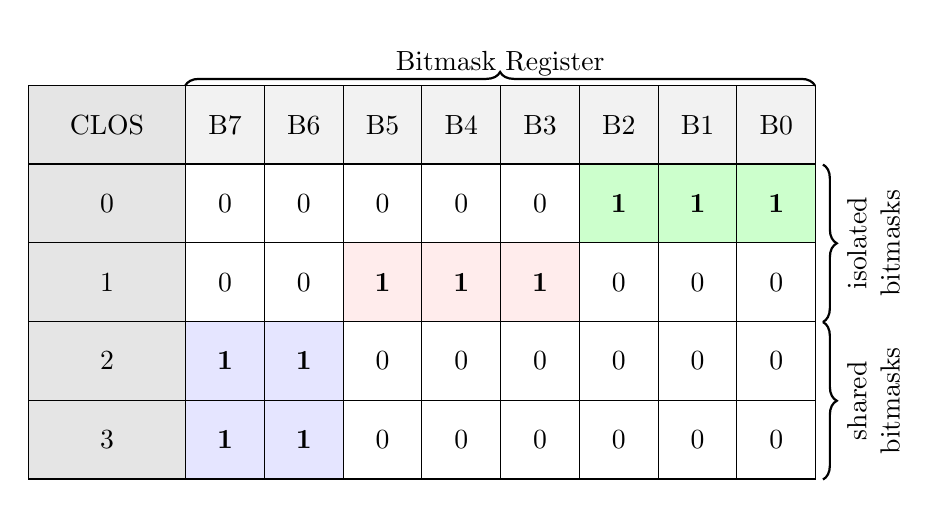
\begin{tikzpicture}

	\foreach \x [evaluate = \bindex using int(8-\x)] in {1,...,8}
		    	\node at (\x,4)[rectangle, draw=black, fill=black!5, minimum height = 1cm, minimum width = 1cm, anchor=south west] (r1\x) 
							{B\bindex};

	\foreach \x in {1,...,8}
				{\ifthenelse{\x>5}
						{\node at (\x,3)[rectangle, draw=black, fill=green!20, minimum height = 1cm, minimum width = 1cm, anchor=south west] (r2\x) {\textbf{1}};}
						{\node at (\x,3)[rectangle, draw=black, fill=white, minimum height = 1cm, minimum width = 1cm, anchor=south west] (r2\x) {0};}

				}
	
		    	%\node at (\x,3)[rectangle, draw=black, fill=white, minimum height = 1cm, minimum width = 1cm, anchor=south west] (r2\x) 
				%			{\ifthenelse{\x>5}{\textbf{1}}{0}};

	\foreach \x in {1,...,8}
				{\ifthenelse{\x>2 \AND \x<6}
						{\node at (\x,2)[rectangle, draw=black, fill=pink!30, minimum height = 1cm, minimum width = 1cm, anchor=south west] (r3\x) {\textbf{1}};}
						{\node at (\x,2)[rectangle, draw=black, fill=white, minimum height = 1cm, minimum width = 1cm, anchor=south west] (r3\x) {0};}
				}
	
		
		    	%% \node at (\x,2)[rectangle, draw=black, fill=white, minimum height = 1cm, minimum width = 1cm, anchor=south west] (r3\x) 
				%%			{\ifthenelse{\x>2 \AND \x<6}{\textbf{1}}{0}};

	\foreach \x in {1,...,8}
				{\ifthenelse{\x<3}
						{\node at (\x,1)[rectangle, draw=black, fill=Blue!10, minimum height = 1cm, minimum width = 1cm, anchor=south west] (r4\x) {\textbf{1}};}
						{\node at (\x,1)[rectangle, draw=black, fill=white, minimum height = 1cm, minimum width = 1cm, anchor=south west] (r4\x) {0};}

				}		    
				%% \node at (\x,1)[rectangle, draw=black, fill=white, minimum height = 1cm, minimum width = 1cm, anchor=south west] (r4\x) 
				%% 			{\ifthenelse{\x<3}{\textbf{1}}{0}};


	\foreach \x in {1,...,8}
				{\ifthenelse{\x<3}
						{\node at (\x,0)[rectangle, draw=black, fill=Blue!10, minimum height = 1cm, minimum width = 1cm, anchor=south west] (r5\x) {\textbf{1}};}
						{\node at (\x,0)[rectangle, draw=black, fill=white, minimum height = 1cm, minimum width = 1cm, anchor=south west] (r5\x) {0};}

				}	
		    	%% \node at (\x,0)[rectangle, draw=black, fill=white, minimum height = 1cm, minimum width = 1cm, anchor=south west] (r5\x) 
				%% 			{\ifthenelse{\x<3}{\textbf{1}}{0}};


	\foreach \y [evaluate = \closindex using int(3-\y)] in {4,...,0}
		    	\node at (-1,\y)[rectangle, draw=black, fill=black!10, minimum height = 1cm, minimum width = 2cm, anchor=south west] (r6\y) 
							{\ifthenelse{\y=4}{CLOS}{\closindex}};

	\draw[thick, decorate, decoration={brace,mirror,amplitude=5pt}] (9.1,2) -- (9.1,4) node [below, align=center, midway, rotate=90, text width=2cm] {\\isolated bitmasks};
	\draw[thick, decorate, decoration={brace,mirror,amplitude=5pt}] (9.1,0) -- (9.1,2) node [below, align=center, midway, rotate=90, text width=2cm] {\\shared bitmasks};

	\draw[thick, decorate, decoration={brace,amplitude=5pt}] (1,5) -- (9,5) node [above, align=center, midway] {\\Bitmask Register};

	%\node (isolatedmasks) at (11, 3) [text width=3cm, align=right]{Isolated Bitmasks};
	%\node (sharedmasks) at (11, 1) [text width=3cm, align=right]{Shared Bitmasks};	

	%\begin{scope}[>=latex]
	%\draw [thick, ->] (r28) to [bend left=45] (isolatedmasks.center);
	%\draw [thick, ->] (r38) to [bend left=45] (isolatedmasks.center);
	%\end{scope}

\end{tikzpicture}
\end{center}
\ifreport
\caption{Example of LLC Partitioning via Bitmasks. Three cache partitions are created by the bitmask registers. 
		First two are isolated ($3/8$ of LLC each) from the rest and the third is shared ($1/4$ of LLC).}
\fi
\label{fig-cat-bitmasks}
\end{figure}

	\endgroup
\end{frame}

\begin{frame}{Features for Efficient Virtualization} {Cache Allocation}
 	\begingroup
	\tikzset{every picture/.style={scale=0.7}, every node/.style={scale=0.7}}	
	\begin{figure}[!htb]
\begin{center}
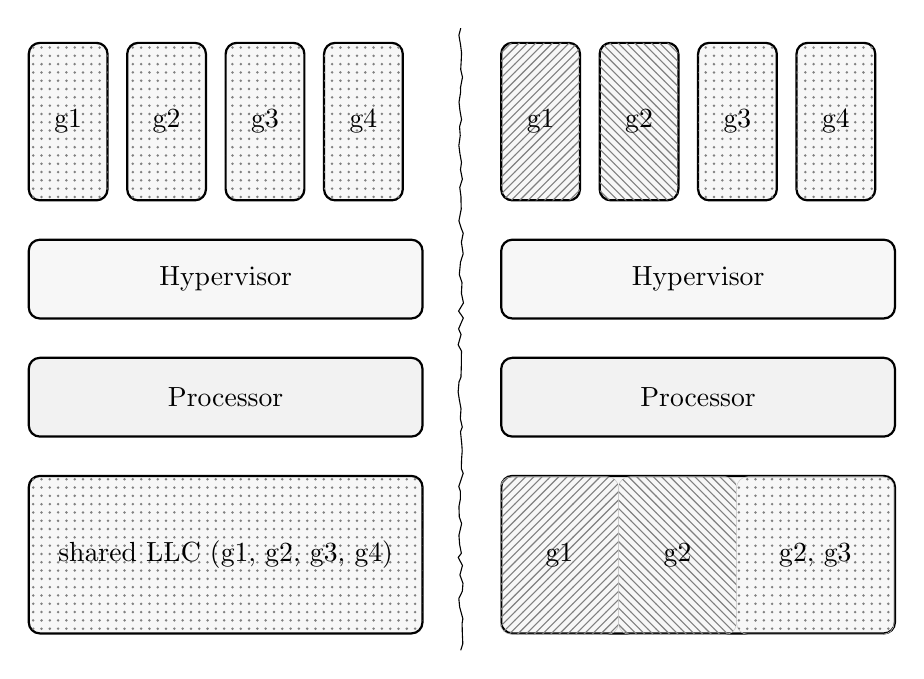
\begin{tikzpicture}


%\draw[step=0.5cm, gray, very thin] (0,0) grid (9,9);


\node at (0,5.5) [rectangle, draw=black, thick, fill=black!3, rounded corners,  postaction={pattern= dots, pattern color=black!50}, minimum height = 2cm, minimum width = 1cm, anchor=south west] (g1) {g1};
\node at (1.25,5.5) [rectangle, draw=black, fill=black!3, thick, rounded corners, postaction={pattern=  dots, pattern color=black!50}, minimum height = 2cm, minimum width = 1cm, anchor=south west] (g2) {g2};
\node at (2.5,5.5) [rectangle, draw=black, fill=black!3, thick, rounded corners, postaction={pattern= dots, pattern color=black!50}, minimum height = 2cm, minimum width = 1cm, anchor=south west] (gN) {g3};
\node at (3.75,5.5) [rectangle, draw=black, fill=black!3, thick, rounded corners, postaction={pattern=  dots, pattern color=black!50}, minimum height = 2cm, minimum width = 1cm, anchor=south west] (gN) {g4};

\node at (6,5.5) [rectangle, draw=black, fill=black!3, thick, rounded corners, postaction={pattern= north east lines, pattern color=black!50}, minimum height = 2cm, minimum width = 1cm, anchor=south west] (g1) {g1};
\node at (7.25,5.5) [rectangle, draw=black, fill=black!3, thick, rounded corners, postaction={pattern= north west lines, pattern color=black!50}, minimum height = 2cm, minimum width = 1cm, anchor=south west] (g2) {g2};
\node at (8.5,5.5) [rectangle, draw=black, fill=black!3, thick, rounded corners, postaction={pattern= dots, pattern color=black!50}, minimum height = 2cm, minimum width = 1cm, anchor=south west] (gN) {g3};
\node at (9.75,5.5) [rectangle, draw=black, fill=black!3, thick, rounded corners, postaction={pattern= dots, pattern color=black!50}, minimum height = 2cm, minimum width = 1cm, anchor=south west] (gN) {g4};

\node at (0,4) [rectangle, draw=black, thick, rounded corners, fill=black!3, minimum height = 1cm, minimum width = 5cm, anchor=south west] (hypervisor1) {Hypervisor} ;
\node at (6,4) [rectangle, draw=black, thick, rounded corners, fill=black!3, minimum height = 1cm, minimum width = 5cm, anchor=south west] (hypervisor2) {Hypervisor} ;

\node at (0,2.5) [rectangle, draw=black, thick, rounded corners, fill=black!5, minimum height = 1cm, minimum width = 5cm, anchor=south west] (cores2) {Processor};
\node at (6,2.5) [rectangle, draw=black, thick, rounded corners, fill=black!5, minimum height = 1cm, minimum width = 5cm, anchor=south west] (cores2) {Processor};

\node at (0,0) [rectangle, draw=black, thick, fill=black!3, rounded corners, postaction={pattern= dots, pattern color=black!50}, minimum height = 2cm, minimum width = 5cm, anchor=south west] (llc1) {shared LLC (g1, g2, g3, g4)};
\node at (6,0) [rectangle, draw=black, thick, rounded corners, fill=black!3, minimum height = 2cm, minimum width = 5cm, anchor=south west] (llc2) {};

\node at (6,0) [rectangle, draw=black!20, very thin, rounded corners, postaction={pattern= north east lines, pattern color=black!50}, minimum height = 2cm, minimum width = 1.5cm, anchor=south west] (g1llc) {g1};
\node at (7.5,0) [rectangle, draw=black!20,  very thin, rounded corners,postaction={pattern= north west lines, pattern color=black!50}, minimum height = 2cm, minimum width = 1.5cm, anchor=south west] (g2llc) {g2};
\node at (9,0) [rectangle, draw=black!20,  very thin, rounded corners,  postaction={pattern= dots, pattern color=black!50}, minimum height = 2cm, minimum width = 2cm, anchor=south west] (g23llc) {g2, g3};

\draw [decorate, decoration={random steps,segment length=3pt,amplitude=1pt}] (5.5,-0.2) -- (5.5,7.7);

\end{tikzpicture}
\end{center}
\ifreport
\caption{Comparison of shared and isolated LLC. One the left is virtual setup when LLC is shared by four guests. On the right is a virtual setup that uses bitmasks from Figure \ref{fig-cat-bitmasks}}
\fi
\label{fig-cat-isolated}
\end{figure}

	\endgroup
\end{frame}

%%%%%%%%%%%%%%%%%~~~SUB SECTION~~~%%%%%%%%%%%%%%%%%
\subsection{PHIDIAS Hypervisor}
\begin{frame}{PHIDIAS Hypervisor}{Design Principles and Features}
  \begin{itemize}
  \item {principle of staticity: static page-tables} \pause{}
  \item {multikernel and microkernel} \pause{}
  \item {static resource allocation} \pause{}
 	\begingroup
	\tikzset{every picture/.style={scale=0.7}, every node/.style={scale=0.7}}	
	\begin{figure}[!htb]
\begin{center}
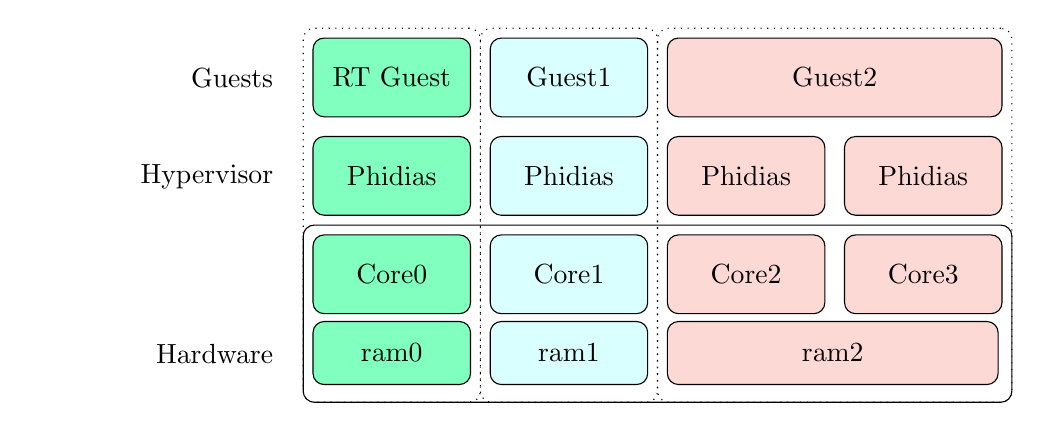
\begin{tikzpicture}

\node at (0,0)[rectangle, draw=black, fill=SpringGreen!50, rounded corners, minimum height = 1cm, minimum width = 2cm, anchor=south west] (core0) {Core0};
\node at (2.25,0)[rectangle, draw=black, fill=Cyan!15, rounded corners, minimum height = 1cm, minimum width = 2cm, anchor=south west] (core1) {Core1};
\node at (4.50,0)[rectangle, draw=black, fill=Salmon!30, rounded corners, minimum height = 1cm, minimum width = 2cm, anchor=south west] (core2) {Core2};
\node at (6.75,0)[rectangle, draw=black, fill=Salmon!30, rounded corners, minimum height = 1cm, minimum width = 2cm, anchor=south west] (core3) {Core3};

\node at (0,-0.9) [rectangle, draw=black, fill=SpringGreen!50, rounded corners, minimum height = 0.8cm, minimum width = 2cm, anchor=south west] (ram0) {ram0};
\node at (2.25,-0.9) [rectangle, draw=black, fill=Cyan!15, rounded corners, minimum height = 0.8cm, minimum width = 2cm, anchor=south west] (ram1) {ram1};
\node at (4.50,-0.9) [rectangle, draw=black, fill=Salmon!30, rounded corners, minimum height = 0.8cm, minimum width = 4.2cm, anchor=south west] (ram2) {ram2};

\begin{scope}[fill opacity=0.0]
\node at (-0.125,-0.125-1)[rectangle, draw=black, fill=white, rounded corners, minimum height = 2.25cm, minimum width = 9.00cm, anchor=south west] (hardware) {};

\node at (-0.125,-1.125)[rectangle, draw=black, fill=black!5, dotted, rounded corners, minimum height = 4.75cm, minimum width = 2.25cm, anchor=south west] (rtg) {};
\node at (2.125,-1.125)[rectangle, draw=black, fill=black!2, dotted, rounded corners, minimum height = 4.75cm, minimum width = 2.25cm, anchor=south west] (g1) {};
\node at (4.375,-1.125)[rectangle, draw=black, fill=black!6, dotted, rounded corners, minimum height = 4.75cm, minimum width = 4.50cm, anchor=south west] (g2) {};

\end{scope}

\node at (0.0,1.25)[rectangle, draw=black, fill=SpringGreen!50, rounded corners, minimum height = 1cm, minimum width = 2cm, anchor=south west] {Phidias};
\node at (2.25,1.25)[rectangle, draw=black, fill=Cyan!15, rounded corners, minimum height = 1cm, minimum width = 2cm, anchor=south west] {Phidias};
\node at (4.50,1.25)[rectangle, draw=black, fill=Salmon!30, rounded corners, minimum height = 1cm, minimum width = 2cm, anchor=south west] {Phidias};
\node at (6.75,1.25)[rectangle, draw=black, fill=Salmon!30, rounded corners, minimum height = 1cm, minimum width = 2cm, anchor=south west] {Phidias};

\node at (0.0,2.5)[rectangle, draw=black, fill=SpringGreen!50, rounded corners, minimum height = 1cm, minimum width = 2cm, anchor=south west] {RT Guest};
\node at (2.25,2.5)[rectangle, draw=black, fill=Cyan!15, rounded corners, minimum height = 1cm, minimum width = 2cm, anchor=south west] {Guest1};
\node at (4.50,2.5)[rectangle, draw=black, fill=Salmon!30, rounded corners, minimum height = 1cm, minimum width = 4.25cm, anchor=south west] {Guest2};

\node (hardware) at (-2.0, -0.5) [text width=3cm, align=right]{Hardware};
\node (phidias) at (-2.0, 1.75) [text width=3cm, align=right]{Hypervisor};
\node (guests) at (-2.0, 3.0) [text width=3cm, align=right]{Guests};

\end{tikzpicture}
\end{center}
\ifreport
\caption{Example partitioning of a multicore x86 platform using Phidias. The guests are allocated separate CPU cores and RAM memory. 
Since Phidias follows multikernel design approach, an instance of Phidias runs on each core.}
\fi
\label{fig-static-part}
\end{figure}

	\endgroup
	\pause{}
  \item {non-preemptive kernel} \pause{}
  \item {low complexity, small footprint and TCB} \pause{}
  \item {support faithful virtualization (x86: VT-x)} \pause{}
  \item {inter-VM communication} \pause{}
  \item {emulated devices: interrupt controller, timer, and UART}
  \end{itemize}
\end{frame}

\begin{frame}{PHIDIAS Hypervisor}{Device Handling}
	\begingroup
	\tikzset{every picture/.style={scale=0.8}, every node/.style={scale=0.8}}	
	\begin{figure}[!htb]
\begin{center}
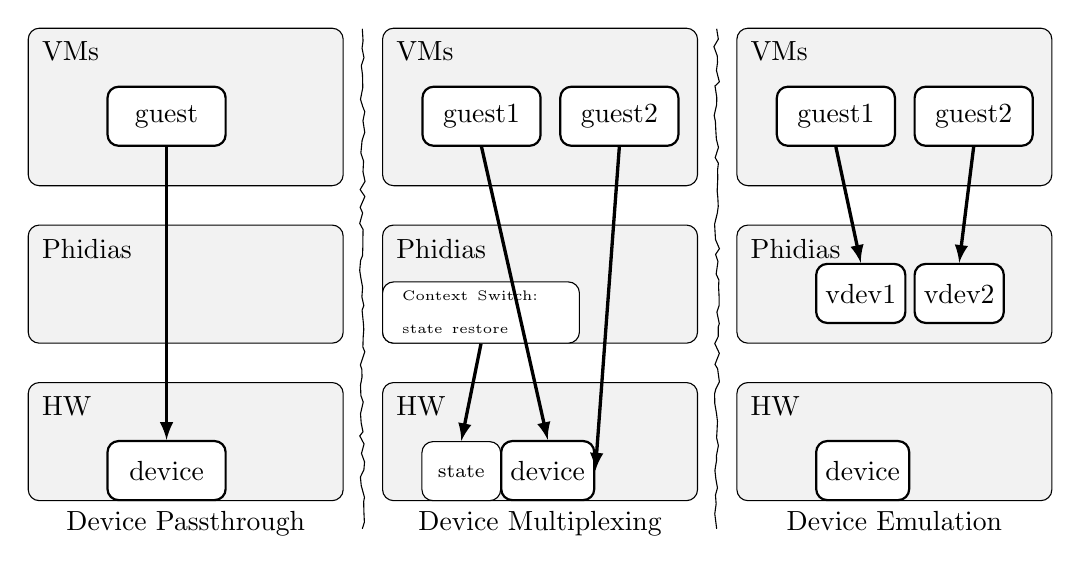
\begin{tikzpicture}

\node at (0,4)[rectangle, draw=black, fill=black!5, rounded corners, minimum height = 2cm, minimum width = 4cm, anchor=south west] (vms1) {};
\node[below right, inner sep=5pt] at (vms1.north west) {VMs};
\node at (4.5,4)[rectangle, draw=black, fill=black!5, rounded corners, minimum height = 2cm, minimum width = 4cm, anchor=south west] (vms2) {};
\node[below right, inner sep=5pt] at (vms2.north west) {VMs};
\node at (9,4)[rectangle, draw=black, fill=black!5, rounded corners, minimum height = 2cm, minimum width = 4cm, anchor=south west] (vms3) {};
\node[below right, inner sep=5pt] at (vms3.north west) {VMs};

\node at (0,2)[rectangle, draw=black, fill=black!5, rounded corners, minimum height = 1.5cm, minimum width = 4cm, anchor=south west] (phidias1) {};
\node[below right, inner sep=5pt] at (phidias1.north west) {Phidias};
\node at (4.5,2)[rectangle, draw=black, fill=black!5,  rounded corners, minimum height = 1.5cm, minimum width = 4cm, anchor=south west] (phidias2) {};
\node[below right, inner sep=5pt] at (phidias2.north west) {Phidias};
\node at (9,2)[rectangle, draw=black, fill=black!5, rounded corners, minimum height = 1.5cm, minimum width = 4cm, anchor=south west] (phidias3) {};
\node[below right, inner sep=5pt] at (phidias3.north west) {Phidias};

\node at (0,0)[rectangle, draw=black, fill=black!5, rounded corners, minimum height = 1.5cm, minimum width = 4cm, label=south:Device Passthrough,anchor=south west] (hw1) {};
\node[below right, inner sep=5pt] at (hw1.north west) {HW};
\node at (4.5,0)[rectangle, draw=black, fill=black!5, rounded corners, minimum height = 1.5cm, minimum width = 4cm, label=south:Device Multiplexing, anchor=south west] (hw2) {};
\node[below right, inner sep=5pt] at (hw2.north west) {HW};
\node at (9,0)[rectangle, draw=black, fill=black!5, rounded corners, minimum height = 1.5cm, minimum width = 4cm, label=south:Device Emulation, anchor=south west] (hw3) {};
\node[below right, inner sep=5pt] at (hw3.north west) {HW};

\node at (1,4.5)[thick, rectangle, draw=black, fill=white, rounded corners, minimum height = 0.75cm, minimum width = 1.5cm, anchor=south west] (g11) {guest};
\node at (1,0)[thick, rectangle, draw=black, fill=white, rounded corners, minimum height = 0.75cm, minimum width = 1.5cm, anchor=south west] (dev1) {device};
\begin{scope}[>=latex]
	\draw [very thick, ->] (g11.south) to [bend right=0] (dev1.north);
\end{scope}

\node at (5,4.5)[thick, rectangle, draw=black, fill=white, rounded corners, minimum height = 0.75cm, minimum width = 1.5cm, anchor=south west] (g21) {guest1};
\node at (6.75,4.5)[thick, rectangle, draw=black, fill=white, rounded corners, minimum height = 0.75cm, minimum width = 1.5cm, anchor=south west] (g22) {guest2};
\node at (4.5,2.0)[rectangle, draw=black, fill=white,  rounded corners, minimum height = 0.75cm, minimum width = 2.5cm, text width=2cm, anchor=south west] (hyp2st) 
					{\tiny{Context Switch: state restore}};
\node at (5,0)[rectangle, draw=black, fill=white, rounded corners, minimum height = 0.75cm, minimum width = 1cm, anchor=south west] (dev2st) {\scriptsize{state}};
\node at (6,0)[thick, rectangle, draw=black, fill=white, rounded corners, minimum height = 0.75cm, minimum width = 1cm, anchor=south west] (dev2) {device};
\begin{scope}[>=latex]
	\draw [very thick, ->] (g21.south) to [bend right=0] (dev2.north);
	\draw [very thick, ->] (g22.south) to [bend right=0] (dev2.east);
	\draw [very thick, ->] (hyp2st.south) to [bend right=0] (dev2st.north);
\end{scope}


\node at (9.5,4.5)[thick, rectangle, draw=black, fill=white, rounded corners, minimum height = 0.75cm, minimum width = 1.5cm, anchor=south west] (g31) {guest1};
\node at (11.25,4.5)[thick, rectangle, draw=black, fill=white, rounded corners, minimum height = 0.75cm, minimum width = 1.5cm, anchor=south west] (g32) {guest2};
\node at (10,2.25)[thick, rectangle, draw=black, fill=white, rounded corners, minimum height = 0.75cm, minimum width = 1cm, anchor=south west] (vdev1) {vdev1};
\node at (11.25,2.25)[thick, rectangle, draw=black, fill=white, rounded corners, minimum height = 0.75cm, minimum width = 1cm, anchor=south west] (vdev2) {vdev2};
\node at (10,0)[thick, rectangle, draw=black, fill=white, rounded corners, minimum height = 0.75cm, minimum width = 1cm, anchor=south west] (dev3) {device};
\begin{scope}[>=latex]
	\draw [very thick, ->] (g31.south) to [bend right=0] (vdev1.north);
	\draw [very thick, ->] (g32.south) to [bend right=0] (vdev2.north);	
\end{scope}

\draw [decorate, decoration={random steps, segment length=3pt,amplitude=1pt}] (4.25,-0.35) -- (4.25,6);
\draw [decorate, decoration={random steps, segment length=3pt,amplitude=1pt}] (8.75,-0.35) -- (8.75,6);

\end{tikzpicture}
\end{center}
\ifreport
\caption{Device handling mechanisms supported by Phidias}
\fi
\label{fig-device-handling}
\end{figure}

	\endgroup
\end{frame}

%%%%%%%%%%%%%%%%%~~~...SECTION...~~~%%%%%%%%%%%%%%%%%
\section{Virtualization Overhead Analysis}
\subsection{Keymetric}
\begin{frame}{Keymetric}
  \begin{itemize}
  \item {interrupt latency or interrupt response time (IRT)}
  \end{itemize}
  	\begingroup
	\tikzset{every picture/.style={scale=0.8}, every node/.style={scale=0.8}}	
	\begin{figure}[!htb]
\begin{center}
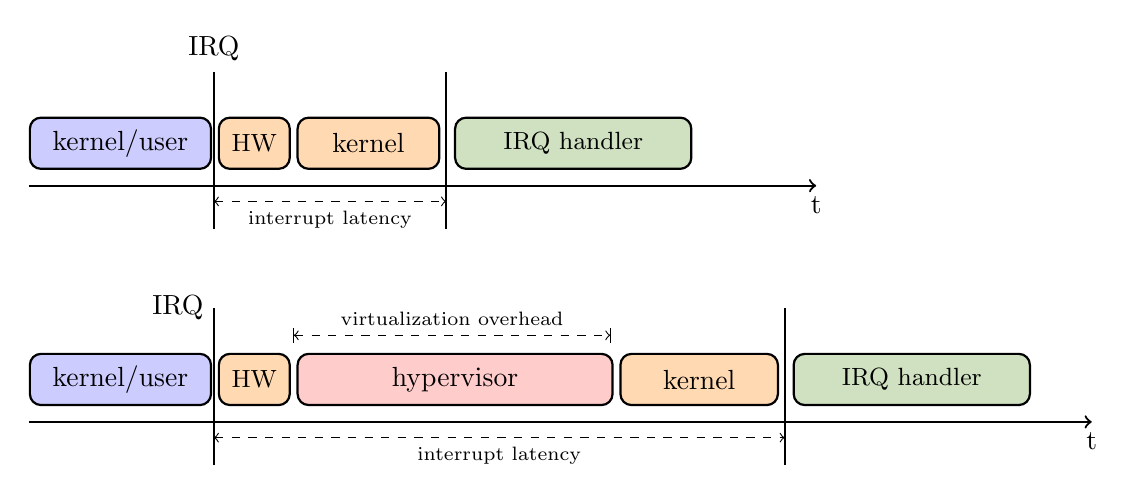
\begin{tikzpicture}

\newcommand\yh{0.65cm}

%\draw[step=1cm, gray, very thin, dotted] (0,0) grid (15,6);

\node at (0,4) [rectangle, draw=black, thick, fill=Blue!20, rounded corners, minimum height = \yh, minimum width = 2.3cm, anchor=south west] (kubefore) 
				{kernel/user};
\node at (2.4,4) [rectangle, draw=black, thick, fill=orange!30, rounded corners, minimum height = \yh, minimum width = 0.9cm, anchor=south west] (hardware) 
				{\small{HW}};
\node at (3.4,4) [rectangle, draw=black, thick, fill=orange!30, rounded corners, minimum height = \yh, minimum width = 1.8cm, anchor=south west] (kservice) {kernel};
\node at (5.4,4) [rectangle, draw=black, thick, fill=OliveGreen!20, rounded corners, minimum height = \yh, minimum width = 3cm, anchor=south west] (kuafter) {\small{IRQ} handler};
\draw[black, thick] (2.35,3.25) -- (2.35,5.25) node [above] {IRQ};
\draw[black, thick] (5.3,3.25) -- (5.3,5.25) node [above] {};
\draw[black, dashed, <->] (2.35,3.6) -- (5.3,3.6) node [below, align=center, midway] {\scriptsize{interrupt latency}};

\draw[black, thick, ->] (0,3.8) -- (10,3.8) node at (10,3.8) [below] {t};

\node at (0,1) [rectangle, draw=black, thick, fill=Blue!20, rounded corners, minimum height = \yh, minimum width = 2.3cm, anchor=south west] (kubefore) {kernel/user};
\node at (2.4,1) [rectangle, draw=black, thick, fill=orange!30, rounded corners, minimum height = \yh, minimum width = 0.9cm, anchor=south west] (hardware) 
				{\small{HW}};

\node at (3.4,1) [rectangle, draw=black, thick, fill=red!20, rounded corners, minimum height = \yh, minimum width = 4cm, anchor=south west] (hyper) {hypervisor};

\node at (7.5,1) [rectangle, draw=black, thick, fill=orange!30, rounded corners, minimum height = \yh, minimum width = 2cm, anchor=south west] (kservice) {kernel};
\node at (9.7,1) [rectangle, draw=black, thick, fill=OliveGreen!20, rounded corners, minimum height = \yh, minimum width = 3cm, anchor=south west] (kuafter) {\small{IRQ} handler};

\draw[black, thick] (2.35,0.25) -- (2.35, 2.25)  node [left] {IRQ};
%\draw[black, thick] (7.4, 0.65) -- (7.4, 2.25) node [above] {};
\draw[black, thick] (9.6,0.25) -- (9.6, 2.25) node [above] {};

\draw[black, dashed, |<->|] (3.35,1.9) -- (7.4,1.9) node [above, align=center, midway] {\scriptsize{virtualization overhead}};
\draw[black, dashed, <->] (2.35,0.6) -- (9.6,0.6) node [below, align=center, midway] {\scriptsize{interrupt latency}};


\draw[black, thick, ->] (0,0.8) -- (13.5,0.8) node at (13.5,0.8) [below] {t};

\end{tikzpicture}
\end{center}
\ifreport
\caption{Interrupt Latency in native and virtualized environment}
\fi
\label{fig-latency-keymetric}
\end{figure}

	\endgroup
\end{frame}

%%%%%%%%%%%%%%%%%~~~SUB SECTION~~~%%%%%%%%%%%%%%%%%
\subsection{Experimental Setup}
\begin{frame}{Experimental Setup} {Virtualization Environment}
  \begin{itemize}
  \item {Hardware  \pause{}
	  \begin{itemize}
	  \item {Xeon E5-2603v4 mounted on ASUS X99E WS motherboard  \pause{}
				\begin{itemize}
				\item {6 CPU cores}  \pause{}
				\item {4GB RAM}  \pause{}
				\item {private 64KB L1 Cache (separate for code, and data)} \pause{} 
				\item {private 512KB L2 Cache}  \pause{}
				\item {shared 15MB L3 Cache}  \pause{}
				%\item {support VT-x  and VT-d (APIC-v, Posted Interrupts, MMU virtualization)}  \pause{}
				\end{itemize}
			}
     \end{itemize}
	}
  \item {PHIDIAS Hypervisor} \pause{}
  \item {Guests: RTOS (preempt\_rt patch) and GPOS (Linux)}
  \end{itemize}
\end{frame}

\begin{frame}{Experimental Setup} {Measurement Setup}
  \begin{itemize}
  \item {PCIe device, FPGA board, External PC}  \pause{}
	\begingroup
	\tikzset{every picture/.style={scale=0.8}, every node/.style={scale=0.8}}	
	\begin{figure}[!htb]
\begin{center}
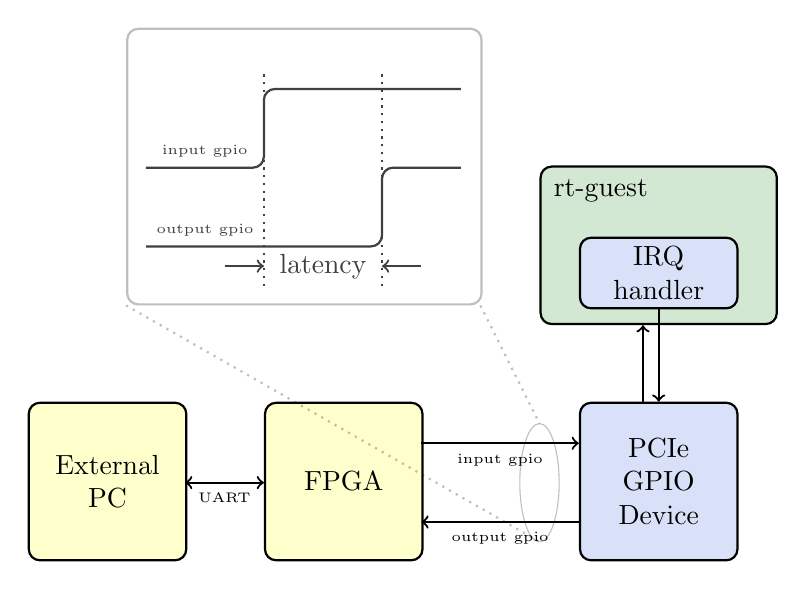
\begin{tikzpicture}

%\draw[step=1cm, gray, very thin, dotted] (0,0) grid (10,8);

\node at (0,0) [rectangle, draw=black, thick, fill=Yellow!20, rounded corners, minimum height = 2cm, minimum width = 2.0cm, align=center, text width=1.7cm, anchor=south west] (pc) 
		{External\\ PC};

\node at (3,0) [rectangle, draw=black, thick, fill=Yellow!20, rounded corners, minimum height = 2cm, minimum width = 2cm, anchor=south west] (fpga) 
		{FPGA};

\node at (7,0) [rectangle, draw=black, thick, fill=RoyalBlue!20, rounded corners, minimum height = 2cm, minimum width = 2cm, align=center, text width=1.7cm, anchor=south west] (pciedev) 
		{PCIe GPIO\\ Device};

\node at (6.5,3) [rectangle, draw=black, thick, fill=ForestGreen!20, rounded corners, minimum height = 2cm, minimum width = 3cm, align=center, text width=1.7cm, anchor=south west] (rtg) {};
\node[below right, inner sep=5pt] at (rtg.north west) {rt-guest};

\node at (7,3.2) [rectangle, draw=black, thick, fill=RoyalBlue!20, rounded corners, minimum height = 0.75cm, minimum width = 2cm, align=center, text width=1.7cm, anchor=south west] (irqhandler) 
		{IRQ handler};

\draw[black, thick, ->] (irqhandler.south) -- (pciedev);
\draw[black, thick, ->] ([xshift=-0.2cm]pciedev.north) -- ([xshift=-0.2cm]rtg.south) ;


\draw[black, thick, <->] (2,1) -- (3,1) node [below, midway, align=center] {\tiny{UART}};
\draw[black, thick, ->] (5,1.5) -- (7,1.5)  node [below, midway, align=center] {\tiny{input gpio}};
\draw[black, thick, <-] (5,0.5) -- (7,0.5)  node [below, midway, align=center] {\tiny{output gpio}};

\draw[black, rounded corners, thick] (1.5,5) -- (3,5) node [above, midway, align=center] {\tiny{input gpio}} -- (3,6) -- (5.5,6);
\draw[black, rounded corners, thick] (1.5,4) -- (4.5,4)  node [above left, midway, align=center] {\tiny{output gpio}} -- (4.5,5) -- (5.5,5);

\draw[black, thick, dotted] (3,3.5) -- (3,6.25);
\draw[black, thick, dotted] (4.5,3.5) -- (4.5,6.25);

\node (latency) at (3.75,3.75) [align=center, text width=1.5cm] {latency};
\draw[black, thick, ->] (2.5,3.75) -- (3,3.75);
\draw[black, thick, <-] (4.5,3.75) -- (5,3.75);

\begin {scope} [opacity=0.25]
\node at (1.25,3.25) [thick, rectangle, draw=black, thick, fill=white, rounded corners, minimum height = 3.5cm, minimum width = 4.5cm, anchor=south west] (lbox) {};
\draw [anchor=south west] {(6.5,1) ellipse (0.25cm and 0.75cm)};
\draw[black, thick, dotted] (1.25,3.25) -- (6.5,0.25);
\draw[black, thick, dotted] (5.75,3.25) -- (6.5,1.75);
\end {scope}


%\node at (1.25,3.25) [thick, ellipse, draw=black, thick, fill=white, rounded corners, minimum height = 1cm, minimum width = 0.5cm, anchor=south west] (gpios) {};

%\draw[black, thick, loosely dotted] (1.5,5) -- (3,5);

\end{tikzpicture}
\end{center}
\ifreport
\caption{Latency measurement setup}
\fi
\label{fig-measure-steup}
\end{figure}

	\endgroup
  \end{itemize}
\end{frame}

%%%%%%%%%%%%%%%%%~~~SUB SECTION~~~%%%%%%%%%%%%%%%%%
\subsection{Methodology}
\begin{frame}{Methodology}{Strategy}
    \begin{itemize}
		%% \item{interrupt source:  \pause{} gpio interrupt  \pause{}
		%%		\begin{itemize}
 		%%		  \item {register gpio IRQ handler in RTOS}   \pause{}
		%%		  \item {IRQ handler responds by assertion of output gpio}   \pause{}
		%%		\end{itemize}
	  	%% 	 }
		\item{compare gpio interrupt latency in: 
				\begin{itemize}
				  \item {native setup} 
				  \item {virtual setup}
				\end{itemize}
            }   \pause{}
        \item{10k interrupts, frequency $@~2ms$} \pause{}
        \item{use synthetic benchmarks to increase confidence} \pause{}
			\begin{itemize}
				\item {executed in rt-guest}
			\end{itemize}
    \end{itemize}
\end{frame}

\begin{frame}{Methodology}{Benchmarks}
	\begin{table}[!htb]
	\centering
	\begin{tabular}{|r|p{6cm}|}  
	\hline
	& \\
	\textbf{Microbenchmark} & \textbf{Description} \\ \hline 
	\mcachepressure{} & processes big data arrays to add pressure on the caches\\ \hline
	\mforkops{} 	& exercises fork operation from userspace\\ \hline
	\mfileops{} 	& exercises file operations from userspace \\ \hline
	\mhackbench{} 	& adds load on kernel scheduler \\ \hline
                                                                       %\tablefootnote{hackbench -p -s1024 -l10000}. \\ \hline
	\mmmapops{} 	& exercises memory map operations \\ \hline
	\mstdout{} 		& exercises data output operations null device\\ \hline
	\mthreadops{} 	& exercises posix thread operations \\ \hline
                                                                       %\tablefootnote{cyclictest -a -t10 -p80 -n -l100000 -i1000 -q}. \\ \hline
	\mnoload{} 	& no load was added \\ \hline
	\end{tabular}
	\end{table}
\end{frame}

%%%%%%%%%%%%%%%%%~~~SUB SECTION~~~%%%%%%%%%%%%%%%%%
\subsection{Baseline}
\begin{frame}{Baseline}{Native Setup}
  	\begingroup
	\tikzset{every picture/.style={scale=0.8}, every node/.style={scale=0.8}}	
	\begin{figure}[!htb]
\begin{center}
\begin{tikzpicture}



\node at (0,3.325) [rectangle, draw=black, thick, fill=white, rounded corners, minimum height = 3cm, minimum width = 6cm, anchor=south west] (rtguest) {};

%\node[inner sep=0pt, text width=2cm] (rtgtext) at (1.5, 5) {PREEMPT\_RT guest};
\node[below right, inner sep=5pt, text width=2cm] at (rtguest.north west) {PREEMPT\_RT\\ Linux\\ (rt-guest)};
\node[above right, inner sep=5pt] (tux) at (rtguest.south)  {
\includegraphics[width=2cm]{figures/tux.jpg}};
%\node[inner sep=0pt] (tux) at (4.5, 5)  {
\includegraphics[width=2cm]{figures/tux.jpg}};

\node at (0,2.250) [rectangle, draw=black, thick, fill=white, rounded corners, minimum height = 1cm, minimum width = 6cm, anchor=south west] (core0) {Core0};

\node at (0,1.125) [rectangle, draw=black, thick, fill=white, rounded corners, minimum height = 1cm, minimum width = 2.875cm, anchor=south west] (lapic) {LAPIC};
\node at (3,1.125) [rectangle, draw=black, thick, fill=white, rounded corners, minimum height = 1cm, minimum width = 3cm, anchor=south west] (ioapic) {IOAPIC};
\node at (0,0) [rectangle, draw=black, thick, fill=white, rounded corners, minimum height = 1cm, minimum width = 2.875cm, anchor=south west] (device) {PCIe Dev.};
\node at (3,0) [rectangle, draw=black, thick, fill=white, rounded corners, minimum height = 1cm, minimum width = 3cm, anchor=south west] (uart) {UART};


\end{tikzpicture}
\end{center}
\ifreport
\caption{Native Setup used to measure baseline interrupt latency}
\fi
\label{fig-native}
\end{figure}

	\endgroup
\end{frame}

\begin{frame}{Baseline} {Interrupt Latency}
  	%\begingroup
	%\tikzset{every picture/.style={scale=0.8}, every node/.style={scale=0.8}}	
	\begin{figure}[!htbp]
\begin{center}
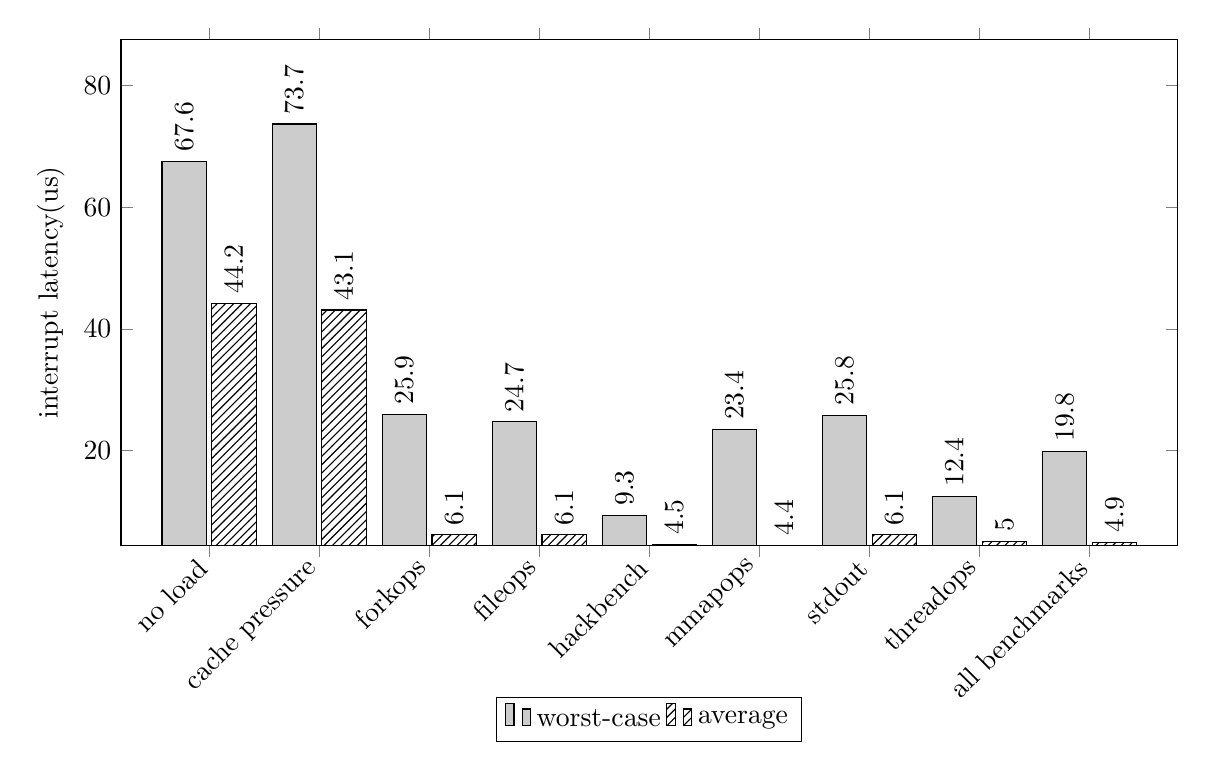
\begin{tikzpicture} %[scale=1.2]

\begin{axis} [ ybar=2pt, height=8cm, width=15cm, enlarge y limits={upper,value=0.2}, %enlargelimits=0.1,
                       legend style={at={(0.5,-0.3)}, anchor=north, legend columns=-1},
                       ylabel={interrupt latency(us)}, %title=vmexits after bootup, 
		       bar width=16pt,
       		       %%enlarge x limits={abs=0.8cm}, 		       
                       symbolic x coords={no load, cache pressure,forkops, fileops, hackbench, mmapops, stdout, threadops, all benchmarks},
                       xtick=data, nodes near coords, 
		       %nodes near coords align={vertical},
			%ymajorgrids=true, grid style = very thin,
		       every node near coord/.append style={rotate=90, anchor=west},
                       x tick label style={rotate=45,anchor=east}, ]                    

	\addplot [fill=black!20] coordinates {
				(no load, 67.6)				
				(cache pressure, 73.7)
				(forkops, 25.9)
				(fileops, 24.7)
				(hackbench, 9.3)
				(mmapops, 23.4)
				(stdout, 25.8)
				(threadops, 12.4)		
				(all benchmarks, 19.8)				
			    };

	\addplot [postaction={pattern=north east lines}] coordinates {
				(no load, 44.2)
				(cache pressure, 43.1)
				(forkops, 6.1)
				(fileops, 6.1)
				(hackbench, 4.5)
				(mmapops, 4.4)
				(stdout, 6.1)
				(threadops, 5.0)
				(all benchmarks, 4.9)		
			    };

\legend{worst-case, average}
\end{axis}

\end{tikzpicture}
\end{center}
\ifreport
\caption{Baseline Interrupt Latency}
\fi
\label{plot-baseline}
\end{figure}

	%\endgroup
\end{frame}

\subsection{Virtualization Overhead}
\begin{frame}{Virtualization Overhead} {Virtual Setup}
  	\begingroup
	\tikzset{every picture/.style={scale=0.7}, every node/.style={scale=0.7}}	
	\begin{figure}[!htb]
\begin{center}
\begin{tikzpicture}

%\node at (0,5.625) [rectangle, draw=black, thick, fill=white, rounded corners, minimum height = 3cm, minimum width = 4cm, text width=2cm, anchor=south west] (rtguest) {};

\node at (0,2.25) [rectangle, draw=black, thick, fill=white, rounded corners, minimum height = 6cm, minimum width = 5cm, anchor=south west] (rtguest) {};

%\node[inner sep=0pt, text width=3cm] (rtgtext) at (2, 8) {PREEMPT\_RT guest};
%\node[inner sep=0pt] (tux) at (3, 7)  {
\includegraphics[width=1.5cm]{figures/tux.jpg}};
\node[below right, inner sep=5pt, text width=2cm] at (rtguest.north west) {PREEMPT\_RT\\ Linux\\ (rt-guest)};
\node[below left, inner sep=2pt] (tux1) at (rtguest.north east)  {
\includegraphics[width=1.8cm]{figures/tux.jpg}};


\node at (0.5,5.1) [rectangle, draw=black, thick, fill=black!5, rounded corners, minimum height = 0.8cm, minimum width = 4cm, anchor=south west] (vcpu1) {vCPU};
\node at (0.5,4.2) [rectangle, draw=black, thick, fill=black!5, rounded corners, minimum height = 0.8cm, minimum width = 1.9cm, anchor=south west] (vlapic1) {vLAPIC};
\node at (2.5,4.2) [rectangle, draw=black, thick, fill=black!5, rounded corners, minimum height = 0.8cm, minimum width = 2cm, anchor=south west] (vioapic1) {vIOAPIC};
\node at (0.5,3.2) [rectangle, draw=black, thick, fill=black!5, rounded corners, minimum height = 0.8cm, minimum width = 1.9cm, anchor=south west] (vdevice) {vTimer};
\node at (2.5,3.2) [rectangle, draw=black, thick, fill=black!5, rounded corners, minimum height = 0.8cm, minimum width = 2cm, anchor=south west] (vuart1) {vUART};

\node at (0.5,2.25+0.1) [rectangle, draw=black, thick, fill=black!10, rounded corners, minimum height = 0.7cm, minimum width = 4cm, anchor=south west] (vdevice) {\small{PCIe GPIO Device}};

\node at (0,1) [rectangle, draw=black, thick, fill=black!3, rounded corners, minimum height = 1cm, minimum width = 5cm, anchor=south west] (phidias1) {PHIDIAS};
\node at (0,0-0.125) [rectangle, draw=black, thick, fill=black!3, rounded corners, minimum height = 1cm, minimum width = 5cm, anchor=south west] (core0) {Core0};


\draw[black, thick, dashed] (5.25,-0.25) -- (5.25,9); %node at (0,0) [below] {release time};

\node at (5.5,2.25) [rectangle, draw=black, thick, fill=white, rounded corners, minimum height = 6cm, minimum width = 5cm, anchor=south west] (guest) {};
%\node[inner sep=0pt, text width=3cm] (rtgtext) at (7, 8) {guest2};
%\node[inner sep=0pt] (tux) at (7.5, 7)  {
\includegraphics[width=1.5cm]{figures/tux.jpg}};

\node[below right, inner sep=5pt, text width=2cm] at (guest.north west) {Linux\\ (gp-guest)};
\node[below left, inner sep=2pt] (tux2) at (guest.north east)  {
\includegraphics[width=1.8cm]{figures/tux.jpg}};

\node at (6,5.1) [rectangle, draw=black, thick, fill=black!5, rounded corners, minimum height = 0.8cm, minimum width = 4cm, anchor=south west] (vcpu2) {vCPU};
\node at (6,4.2) [rectangle, draw=black, thick, fill=black!5, rounded corners, minimum height = 0.8cm, minimum width = 1.9cm, anchor=south west] (vlapic2) {vLAPIC};

\node at (8,4.2) [rectangle, draw=black, thick, fill=black!5, rounded corners, minimum height = 0.8cm, minimum width = 2cm, anchor=south west] (vioapic2) {vIOAPIC};
\node at (6,3.2) [rectangle, draw=black, thick, fill=black!5, rounded corners, minimum height = 0.8cm, minimum width = 1.9cm, anchor=south west] (vdevice) {vTimer};
\node at (8,3.2) [rectangle, draw=black, thick, fill=black!5, rounded corners, minimum height = 0.8cm, minimum width = 1.9cm, anchor=south west] (vuart2) {vUART};

\node at (5.5,1) [rectangle, draw=black, thick, fill=black!3, rounded corners, minimum height = 1cm, minimum width = 5cm, anchor=south west] (phidias2) {PHIDIAS};
\node at (5.5,0-0.125) [rectangle, draw=black, thick, fill=black!3, rounded corners, minimum height = 1cm, minimum width = 5cm, anchor=south west] (core1) {Core1};


\draw[black, thick, dotted] (-0.25, 2.1) -- (11,2.1);

\end{tikzpicture}
\end{center}
\ifreport
\caption{Virtual Setup used to measure virtualization overhead}
\fi
\label{fig-virtual}
\end{figure}

	\endgroup
\end{frame}

\begin{frame}[allowframebreaks]{Virtualization Overhead} {Interrupt Latency Overhead}
  	%\begingroup
	%\tikzset{every picture/.style={scale=0.8}, every node/.style={scale=0.8}}	
	\begin{figure}[!htb]
\begin{center}
\begin{tikzpicture}

\begin{axis} [name=plot1, height=\figheight, width=\figwidth, ybar=\ybarSepVO, enlarge y limits={upper,value=0.3},  
			ymin=0,
			legend pos=north east, legend columns=-1,
            ylabel={worst-case interrupt latency ($\mu{}s$)}, 
		    bar width=\ybarWidthVO,
			x=\ybarXdistVO,
            symbolic x coords={no load, cache\_pressure,forkops, fileops, hackbench, mmapops, stdout, threadops, all benchmarks},
            xtick=data, nodes near coords, nodes near coords align={vertical}, nodes near coords style={font=\ttfamily\scriptsize},
			x tick label style={rotate=25,anchor=east, font=\ttfamily\small}, ]                    
	\addplot [fill=yellow!20, postaction={pattern=north east lines}, pattern color=gray] coordinates {
				(no load, 67.6)				
				(cache\_pressure, 73.7)
				(forkops, 25.9)
				(fileops, 24.7)
				(hackbench, 9.3)
				(mmapops, 23.4)
				(stdout, 25.8)
				(threadops, 12.4)
				(all benchmarks, 19.8)
			      };

	\addplot [fill=NavyBlue!40] coordinates {
				(no load, 130.8)				
				(cache\_pressure, 141.7)
				(forkops, 119.5)
				(fileops, 146.4)
				(hackbench, 106.7)
				(mmapops, 106.6)
				(stdout, 142.7)
				(threadops, 169.1)
				(all benchmarks, 114.1)
			      };
\legend{native setup, virtual setup}
\end{axis}

%%%%%%%%%%%%%%%%%%for defense presentation%%%%%%%%%%%%%%%%%%%%
\ifdefense

\end{tikzpicture}
\end{center}
\label{plot-native-vs-virtual1}
\end{figure}
	
\begin{figure}[!htb]
\begin{center}
\begin{tikzpicture}

\fi
%%%%%%%%%%%%%%%%%%%%%ENDIF%%%%%%%%%%%%%%%%%%%%%%%%%%%%%%%%%

\begin{axis} [name=plot2,\atCmdVOverheadLowerPlot,  height=\figheight, width=\figwidth, ybar=\ybarSepVO, enlarge y limits={upper,value=0.2}, 
				ymin=0,
                legend pos=north east, legend columns=-1,
                ylabel={average-case interrupt latency ($\mu{}s$)}, 
		       	bar width=\ybarWidthVO,
				x=\ybarXdistVO,
				symbolic x coords={no load, cache\_pressure,forkops, fileops, hackbench, mmapops, stdout, threadops, all benchmarks},
                xtick=data, nodes near coords, nodes near coords align={vertical},  nodes near coords style={font=\ttfamily\scriptsize},
				 x tick label style={rotate=25,anchor=east, font=\ttfamily\small}, ]                    
	\addplot [fill=yellow!20, postaction={pattern=north east lines}, pattern color=gray] coordinates {
				(no load, 44.2)				
				(cache\_pressure, 43.1)
				(forkops, 6.1)
				(fileops, 6.1)
				(hackbench, 4.5)
				(mmapops, 4.4)
				(stdout, 6.1)
				(threadops, 5)
				(all benchmarks, 4.9)
			      };
	\addplot [fill=NavyBlue!40] coordinates {
				(no load, 18.2)				
				(cache\_pressure, 26.6)
				(forkops, 12.6)
				(fileops, 14.3)
				(hackbench, 10)
				(mmapops, 8.1)
				(stdout, 14.9)
				(threadops, 16.4)
				(all benchmarks, 10.2)
			      };
\legend{native setup, virtual setup}
\end{axis}

\end{tikzpicture}
\end{center}
\ifreport
\caption{Comparison of worst-case and average-case latency in native and virtual setup}
\label{plot-native-vs-virtual}
\else
\label{plot-native-vs-virtual2}
\fi
\end{figure}

	%\endgroup
\end{frame}

\begin{frame}{Virtualization Overhead} {Phidias Intervention}

	\begin{table}[H]
	\centering
	\begin{tabular}{|r|c|c|}  
	\hline
    \textbf{load}	&	\textbf{total exits in $30s$}	&	\textbf{exits in $1ms$} (average) \\ \hline
	\mcachepressure{}	&		16987	&	1 	\\ \hline
	\mforkops{}	&			1381087	&	46 		\\ \hline
	\mfileops{}	&			804448	&	27 		\\ \hline
	\mhackbench{}	&		3461504	&	\textbf{115} \\ \hline
	\mmmapops{}	&			174722	&	6		 \\ \hline
	\mstdout{}	&			937329	&	31 		\\ \hline
	\mthreadops{}	&		470481	&	16 		\\ \hline
	\end{tabular}
	\end{table}
\end{frame}

\begin{frame} {Virtualization Overhead} {Overhead Components}
    \begingroup
	\tikzset{every picture/.style={scale=0.8}, every node/.style={scale=0.8}}	
	\begin{figure}[!htb]
\begin{center}
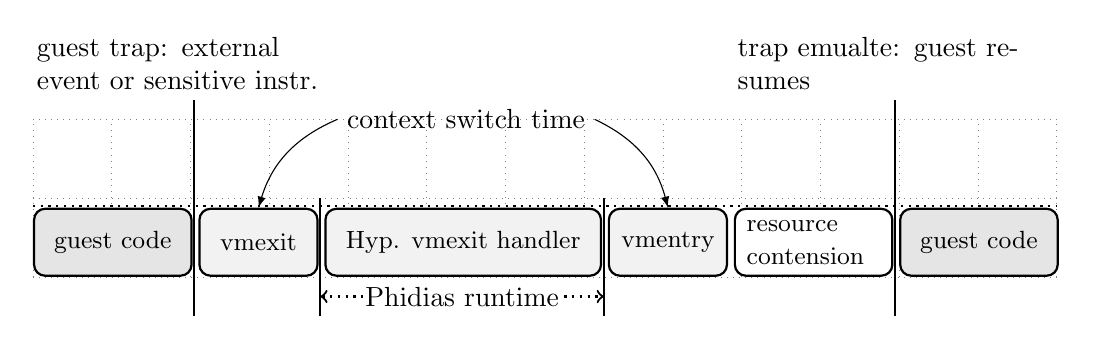
\begin{tikzpicture}

\newcommand\yh{0.85cm}

\draw[step=1cm, gray, very thin, dotted] (0,0) grid (13,2);
\draw[black, thick, dotted] (0,0.9) -- (13,0.9) node at (13,0.9) [below] {};

\node at (0,0) [rectangle, draw=black, thick, fill=black!10, rounded corners, minimum height = \yh, minimum width = 2cm, anchor=south west] (gcbefore) {\small{guest code}};
\node at (2.1,0) [rectangle, draw=black, thick, fill=black!5, rounded corners, minimum height = \yh, minimum width = 1.5cm, anchor=south west] (vmexit) {\small{vmexit}};
\node at (3.7,0) [rectangle, draw=black, thick, fill=black!5, rounded corners, minimum height = \yh, minimum width = 3.5cm, anchor=south west] (phidias) {\small{Hyp. vmexit handler}};
\node at (7.3,0) [rectangle, draw=black, thick, fill=black!5, rounded corners, minimum height = \yh, minimum width = 1.5cm, anchor=south west] (vmentry) {\small{vmentry}};

\node at (8.9,0) [rectangle, draw=black, thick, fill=white, rounded corners, minimum height = \yh, minimum width = 2cm, text width = 1.7cm, anchor=south west] (rc) {\small{resource\\ contension}};

\node at (11.0,0) [rectangle, draw=black, thick, fill=black!10, rounded corners, minimum height = \yh, minimum width = 2cm, anchor=south west] (gcafter) {\small{guest code}};

\draw[black, thick] (2.05,-0.5) -- (2.05, 2.25)  node [above, text width = 4cm] {guest trap: external event or sensitive instr.};
\draw[black, thick] (10.95,-0.5) -- (10.95, 2.25)  node [above, text width = 4cm] {trap emualte: guest resumes};

\draw[black, thick] (3.65,-0.5) -- (3.65, 1);
\draw[black, thick] (7.25,-0.5) -- (7.25, 1);
\draw[black, thick, dotted, <-] (3.65, -0.25) -- (4.25, -0.25); 
\draw[black, thick, dotted, ->] (6.75, -0.25) -- (7.25, -0.25);
\node at (5.45, -0.25) {Phidias runtime};

\node at (5.5, 2) (cslabel) [align=center] {context switch time};

\begin{scope}[>=latex]
	\draw [black, ->] (cslabel.west) to [bend right=25]  (vmexit.north);
	\draw [black, ->] (cslabel.east) to [bend left=25]  (vmentry.north);
\end{scope}

\end{tikzpicture}
\end{center}
\ifreport
\caption{Virtualization overhead components: Phidias runtime, context-switch time and resource contention}
\fi
\label{fig-virt-overhead-all-comp}
\end{figure}

	\endgroup
\end{frame}

\begin{frame}[allowframebreaks] {Overhead Components} {Phidias Runtime}
    \begingroup
	\tikzset{every picture/.style={scale=0.8}, every node/.style={scale=0.8}}	
	\begin{figure}[!htb]
\begin{center}
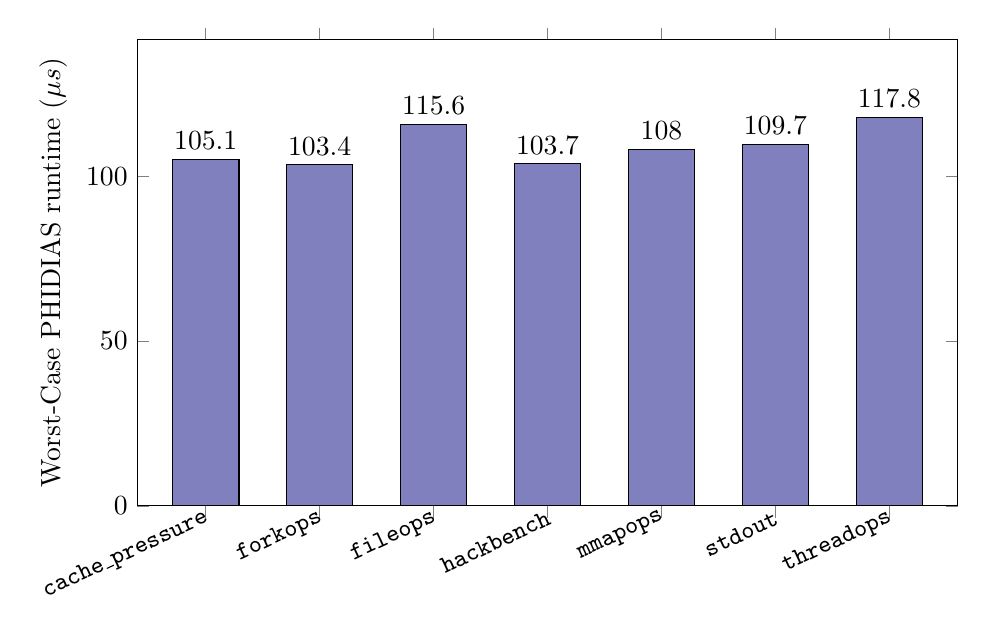
\begin{tikzpicture}

\begin{axis} [ ymin=0, ybar=2pt, height=7.5cm, width=\figwidth, enlarge y limits={upper,value=0.2}, 
		       legend style={at={(0.5,-0.3)}, anchor=north, legend columns=-1},
               ylabel={Worst-Case PHIDIAS runtime ($\mu{}s$)},
		       bar width=24pt,
  		       %%enlarge x limits={abs=0.8cm}, 		       
               symbolic x coords={no load, cache\_pressure,forkops, fileops, hackbench, mmapops, stdout, threadops, all benchmarks},
               xtick=data, nodes near coords, 
		       nodes near coords align={vertical},
		       %every node near coord/.append style={rotate=90, anchor=west},
               x tick label style={rotate=25, anchor=east, xshift=4pt, font=\ttfamily\small}, ]    

			\addplot [fill=NavyBlue!50] coordinates {				
				(cache\_pressure, 105.1)
				(forkops, 103.4)
				(fileops, 115.6)
				(hackbench, 103.7)
				(mmapops, 108)
				(stdout, 109.7)
				(threadops, 117.8)				
			    };
%\legend{}
\end{axis}

\end{tikzpicture}
\ifreport
\caption{Phidias runtime under different load conditions}
\fi
\end{center}
\label{plot-phidias-runtime}
\end{figure}

	\endgroup
\end{frame}

\begin{frame}[allowframebreaks]{Overhead Components} {Phidias Runtime CPI}
	\begin{table}[H]
	\centering
	\begin{tabular}{|c|c|c|c|c|}  
	\hline
							& \multicolumn{2}{|c|}{\textbf{Phidias runtime}} & \textbf{instructions}	& \textbf{CPI} \\
	\textbf{Benchmark}		& average (cc)	&	worst-case (cc)	&	\textbf{retired} (WC) &	(WC) \\ \hline 
	\mcachepressure{}	& 16548	& 178716 & 2322 & 77 \\ \hline
	\mforkops{}		& 9263 & 175702 & 2301 & 76.4 \\ \hline
	\mfileops{}		& 698 & 196490 & 12640 & 15.5 \\ \hline
	\mhackbench{} 		& 23042 & 176205 & 2301 & 76.6 \\ \hline
	\mmmapops{} 		& 7604 & 183566 & 2364 & \textbf{77.7} \\ \hline
	\mstdout{} 			& 1240 & 186435 & 21429 & 8.7 \\ \hline
	\mthreadops{} 		& 1265 & 200313 & 19804 & 10.1 \\ \hline
	\end{tabular}
	\end{table}

	\begin{itemize}
		\item {worst-case CPI is very high}
		\item {difference in average and worst-case is high}
	\end{itemize}
\end{frame}

\begin{frame}[allowframebreaks]{Overhead Components} {Context-Switch time}
	\begingroup
	\tikzset{every picture/.style={scale=0.7}, every node/.style={scale=0.7}}	
	\begin{figure}[!htb]
\begin{center}
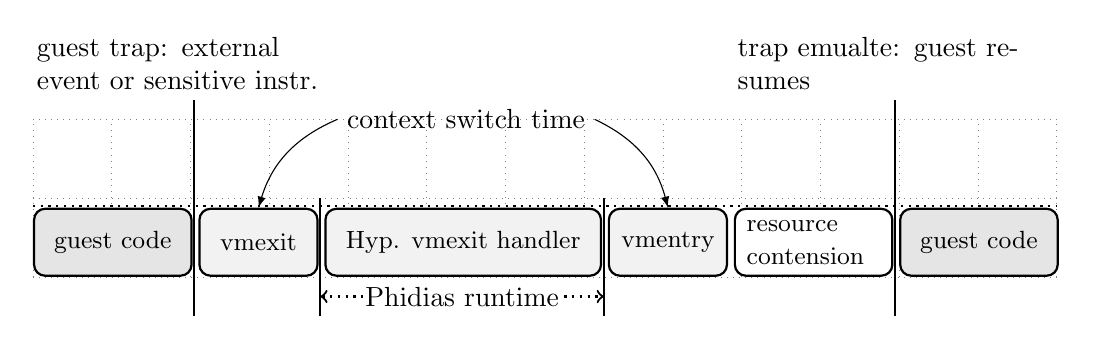
\begin{tikzpicture}

\newcommand\yh{0.85cm}

\draw[step=1cm, gray, very thin, dotted] (0,0) grid (13,2);
\draw[black, thick, dotted] (0,0.9) -- (13,0.9) node at (13,0.9) [below] {};

\node at (0,0) [rectangle, draw=black, thick, fill=black!10, rounded corners, minimum height = \yh, minimum width = 2cm, anchor=south west] (gcbefore) {\small{guest code}};
\node at (2.1,0) [rectangle, draw=black, thick, fill=black!5, rounded corners, minimum height = \yh, minimum width = 1.5cm, anchor=south west] (vmexit) {\small{vmexit}};
\node at (3.7,0) [rectangle, draw=black, thick, fill=black!5, rounded corners, minimum height = \yh, minimum width = 3.5cm, anchor=south west] (phidias) {\small{Hyp. vmexit handler}};
\node at (7.3,0) [rectangle, draw=black, thick, fill=black!5, rounded corners, minimum height = \yh, minimum width = 1.5cm, anchor=south west] (vmentry) {\small{vmentry}};

\node at (8.9,0) [rectangle, draw=black, thick, fill=white, rounded corners, minimum height = \yh, minimum width = 2cm, text width = 1.7cm, anchor=south west] (rc) {\small{resource\\ contension}};

\node at (11.0,0) [rectangle, draw=black, thick, fill=black!10, rounded corners, minimum height = \yh, minimum width = 2cm, anchor=south west] (gcafter) {\small{guest code}};

\draw[black, thick] (2.05,-0.5) -- (2.05, 2.25)  node [above, text width = 4cm] {guest trap: external event or sensitive instr.};
\draw[black, thick] (10.95,-0.5) -- (10.95, 2.25)  node [above, text width = 4cm] {trap emualte: guest resumes};

\draw[black, thick] (3.65,-0.5) -- (3.65, 1);
\draw[black, thick] (7.25,-0.5) -- (7.25, 1);
\draw[black, thick, dotted, <-] (3.65, -0.25) -- (4.25, -0.25); 
\draw[black, thick, dotted, ->] (6.75, -0.25) -- (7.25, -0.25);
\node at (5.45, -0.25) {Phidias runtime};

\node at (5.5, 2) (cslabel) [align=center] {context switch time};

\begin{scope}[>=latex]
	\draw [black, ->] (cslabel.west) to [bend right=25]  (vmexit.north);
	\draw [black, ->] (cslabel.east) to [bend left=25]  (vmentry.north);
\end{scope}

\end{tikzpicture}
\end{center}
\ifreport
\caption{Virtualization overhead components: Phidias runtime, context-switch time and resource contention}
\fi
\label{fig-virt-overhead-all-comp}
\end{figure}

	\endgroup	    
	\begin{table}[H]
	\centering
	\begin{tabular}{|c||c|c|}  
	\hline
		Context-switch time	&	average ($\mu{}s$)	&	worst-case ($\mu{}s$) \\ \hline \hline
		\mnoload{}				&	1			& 		17.2 \\ \hline
		\mcachepressure{}		&	1			& \textbf{86.8}\\ \hline
	\end{tabular}
	\end{table}
\end{frame}

%% \begin{frame}[allowframebreaks]{Overhead Components} {Context-Switch time CDF}
%%    \begingroup
%%	\tikzset{every picture/.style={scale=0.9}, every node/.style={scale=0.9}}	
%%	\begin{figure}[!htb]
\begin{center}

\begin{tikzpicture}


\begin{axis}[name=plot1, height=8cm, width=12cm,
		legend pos=south east,
		xlabel=context-switch overhead ($\mu{}s$), 
		ylabel=Probability, enlargelimits=0.05,
		%ymajorgrids=true, grid style = very thin,
		]
	\addplot [ultra thick, blue] table[x=Latency,y=Probability] {./figures/vmexitentry_10k_cdf.dat};
	\addplot [very thick, red, dashed] table[x=Latency,y=Probability] {./figures/vmexitentry_cachepressure_10k_cdf.dat};
	\legend {\small{no load (max 17.2)}, \small{cache pressure (max 86.8)}}
\end{axis}

\end{tikzpicture}
\end{center}
\ifreport
\caption{CDF of context-switch overhead}
\fi
\label{plot-cdf-contextswitch}
\end{figure}

%%	\endgroup
%% \end{frame}

%% \begin{frame}{VT-x Properties and Real-Time Guests} {non-deterministic behavior}
%%   \begin{itemize}
%%    \item {big multi-level caches} \pause{}
%%    \item {big data structures to manage VMs} \pause{}
%%    \item {unknown instruction behavior (e.g. INVVPID)}
%%   \end{itemize}
%% \end{frame}

%%%%%%%%%%%%%%%%%~~~...SECTION...~~~%%%%%%%%%%%%%%%%%
\section{Latency Reduction Techniques}

\subsection{Direct Interrupt Injection}
\begin{frame} {Direct Interrupt Injection} {Methodology}
    
	\begin{itemize}
      \item {extend Phidias to support DII} \pause {}
      \item {use DII to route gpio interrupt to rt-guest} \pause {}
			\begingroup
			\tikzset{every picture/.style={scale=0.7}, every node/.style={scale=0.7}}	
			\begin{figure}[!htb]
\begin{center}
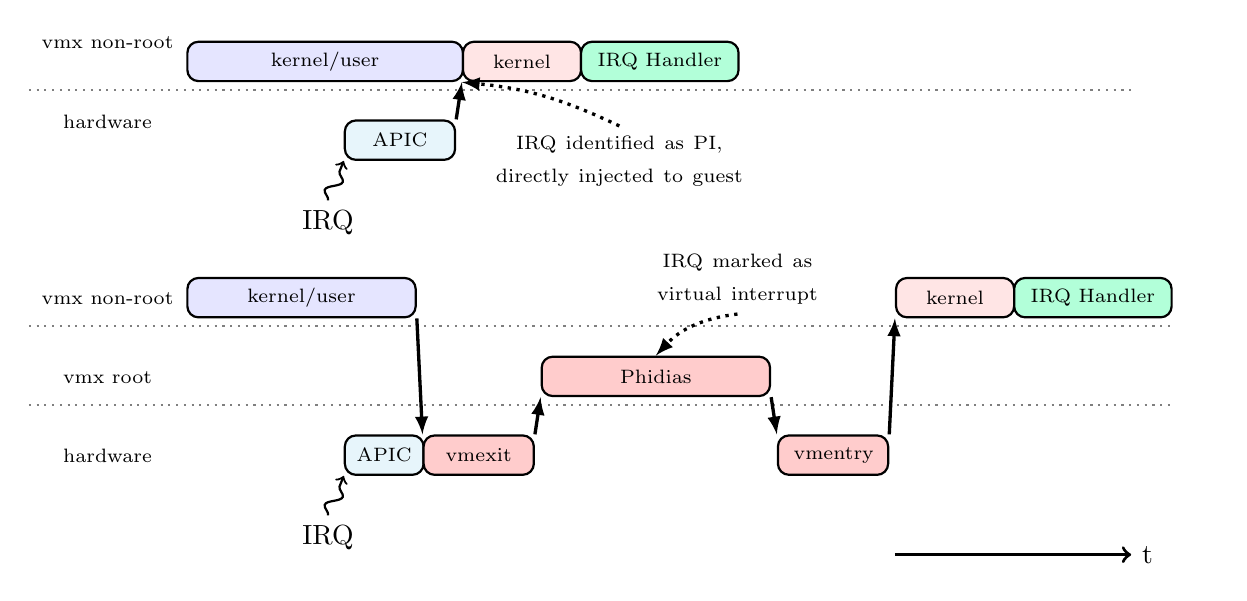
\begin{tikzpicture}

%\draw[step=1cm, gray, very thin, dotted] (-1,-1) grid (10,6);

\draw[black, very thick, ->] (9,-1) -- (12,-1) node [below, right] {t};
\draw[black, thick, dotted, opacity=0.5] (-2,0.9) -- (12.5,0.9) node at (13,0.9) [below] {};
\draw[black, thick, dotted, opacity=0.5] (-2,1.9) -- (12.5,1.9) node at (13,1.9) [below] {};
\node at (-1, 2.25) {\scriptsize{vmx non-root}};
\node at (-1, 1.25) {\scriptsize{vmx root}};
\node at (-1, 0.25) {\scriptsize{hardware}};


\node at (0,2) [rectangle, draw=black, thick, fill=Blue!10, rounded corners, minimum height = 0.5cm, minimum width = 2.9cm, anchor=south west] (kubefore) {\scriptsize{kernel/user}};
%\draw[black, thick, dashed, opacity=0.7] (1.95,-0.25) -- (1.95, 3.0)  node [above, text width = 1cm] {IRQ};
\node at (2,0) [rectangle, draw=black, thick, fill=SkyBlue!20, rounded corners, minimum height = 0.5cm, minimum width = 1cm, anchor=south west] (apic) {\scriptsize{APIC}};
%\draw[black, thick, dashed] (3.0,-0.25) -- (3.0, 3.75)  node [above, text width = 4cm] {IRQ not marked as PI};
\node at (3,0) [rectangle, draw=black, thick, fill=Red!20, rounded corners, minimum height = 0.5cm, minimum width = 1.4cm, anchor=south west] (vmexit) {\scriptsize{vmexit}};
\node at (4.5,1) [rectangle, draw=black, thick, fill=Red!20, rounded corners, minimum height = 0.5cm, minimum width = 2.9cm, anchor=south west] (phidias) {\scriptsize{Phidias}};
\node at (7.5,0) [rectangle, draw=black, thick, fill=Red!20, rounded corners, minimum height = 0.5cm, minimum width = 1.4cm, anchor=south west, text width=1cm] (vmentry) {\scriptsize{vmentry}};
%\draw[black, thick, dashed] (7.5,-0.25) -- (7.5, 3.25)  node [above, text width = 4cm] {IRQ marked pending};
\node at (9,2) [rectangle, draw=black, thick, fill=red!10, rounded corners, minimum height = 0.5cm, minimum width = 1.5cm, anchor=south west] (kafter) {\scriptsize{kernel}};
\node at (10.5,2) [rectangle, draw=black, thick, fill=SpringGreen!30, rounded corners, minimum height = 0.5cm, minimum width = 2cm, anchor=south west] (irqhandler) {\scriptsize{IRQ Handler}};
\draw[thick, decorate, decoration=snake, ->] (1.8, -0.5) -- (2, 0) node at (1.8, -0.5) [below] {IRQ};


\node at (7,2.5) (irqvi) [text width=4cm, align=center] {\scriptsize{IRQ marked as virtual interrupt}};
\node at (5.5,4) (irqpi) [text width=4cm, align=center] {\scriptsize{IRQ identified as PI, directly injected to guest}};

\begin{scope}[>=latex]
	%\draw [thick, ->] (kubefore.south east) to [bend right=0] (vmexit.north west);
	\draw [very thick, ->] (kubefore.south east) -- (vmexit.north west);
	\draw [very thick, ->] (vmexit.north east) -- (phidias.south west);
	\draw [very thick, ->] (phidias.south east) -- (vmentry.north west);
	\draw [very thick, ->] (vmentry.north east) -- (kafter.south west);
	\draw [very thick, dotted, ->] (irqvi.south) to [bend right=20] (phidias.north);
	
\end{scope}

\draw[black, thick, dotted, opacity=0.5] (-2,8-3.1) -- (12,8-3.1) node at (13,8-3.1) [below] {};
\node at (-1, 8-2.5) {\scriptsize{vmx non-root}};
\node at (-1, 8-3.5) {\scriptsize{hardware}};

\node at (0,8-3) [rectangle, draw=black, thick, fill=Blue!10, rounded corners, minimum height = 0.5cm, minimum width = 3.5cm, anchor=south west] (kubefore2) {\scriptsize{kernel/user}};
%\draw[black, thick, dashed, opacity=0.7] (1.95,-4.25) -- (1.95, -2.0)  node [above, text width = 1cm] {IRQ};
\draw[thick, decorate, decoration=snake, ->] (1.8, 8-4.5) -- (2, 8-4) node at (1.8, 8-4.5) [below] {IRQ};
\node at (2.0,8-4) [rectangle, draw=black, thick, fill=SkyBlue!20, rounded corners, minimum height = 0.5cm, minimum width = 1.4cm, anchor=south west] (apic2) {\scriptsize{APIC}};
%\draw[black, thick, dashed] (3.5,-4.25) -- (3.5, -1.5)  node [above, text width = 4cm] {IRQ recognized as PI};

\node at (3.5,8-3) [rectangle, draw=black, thick, fill=red!10, rounded corners, minimum height = 0.5cm, minimum width = 1.5cm, anchor=south west] (kafter2) {\scriptsize{kernel}};
\node at (5.0,8-3) [rectangle, draw=black, thick, fill=SpringGreen!30, rounded corners, minimum height = 0.5cm, minimum width = 2cm, anchor=south west] (irqhandler2) {\scriptsize{IRQ Handler}};

\begin{scope}[>=latex]
	\draw [very thick, ->] (apic2.north east) -- (kafter2.south west);
	\draw [very thick, dotted, ->] (irqpi.north) to [bend right=10] (kafter2.south west);
\end{scope}


\end{tikzpicture}
\end{center}
\ifreport
\caption{Posted interrupt versus virtual interrupt delivery}
\fi
\label{fig-posted-interrupts}
\end{figure}

			\endgroup
			\pause {}
   	  \item {repeat latency measurement experiments} \pause {}
    \end{itemize}
    
\end{frame}

\begin{frame} [allowframebreaks] {Direct Interrupt Injection} {Latency Reduction}
    %\begingroup
	%\tikzset{every picture/.style={scale=1}, every node/.style={scale=1}}	
	\begin{figure}[!htb]
\begin{center}
\begin{tikzpicture} [
						my brace/.style={thick, decorate, decoration={brace, amplitude=4pt, raise=10pt,},},							
						my label/.style={below right, align=center, rotate=90, inner ysep=14pt, },						
					]

	%%%%%%% worst case %%%%%%%%%%%%%%
	\begin{axis} [ name=plot1, height=\figheight, width=\figwidth, 
				   enlarge y limits={upper,value=0.3},  enlarge x limits=0.12,
				   ymin=0,
		           %axis y line*=left,
				   ybar=\ybarSep,  
				   x=\ybarXdist,
				   bar width=\ybarWidth,
	   			   ylabel={worst-case interrupt latency ($\mu{}s$)},
	 		       symbolic x coords={no load, cache\_pressure, forkops, fileops, threadops},
		           xtick=data,                 
		            %nodes near coords, 
					%nodes near coords align={vertical}, 
					x tick label style={rotate=0, anchor=north, font=\ttfamily\small}, 
					%% xticklabel style={rotate=0,anchor=north},
		            xtick align=inside,
		            xticklabel pos=left,
	   			    legend pos=north east, legend columns=-1,
				]     
               
	\addplot [fill=yellow!20, postaction={pattern=north east lines}, pattern color=gray] coordinates {
				(no load, 67.6)				
				(cache\_pressure, 73.7)
				(forkops, 25.9)
				(fileops, 24.7)
				(threadops, 12.4)
		      };

	%% absolute values
	\addplot [fill=NavyBlue!50, xshift=\xShiftLatency] coordinates {
                    (no load,133.9) 
					(cache\_pressure,135.8)	
					(forkops,127.1)
					(fileops,127.6)
					(threadops,131.7)
			      }
					coordinate [pos=0] (a1)
		            coordinate [pos=0.2] (a2)
		            coordinate [pos=0.4] (a3)
		            coordinate [pos=0.8] (a4)
		            coordinate [pos=1] (a5)
				  ;

	\addplot [fill=ForestGreen!60, xshift=\xShiftLatency, postaction={pattern=crosshatch dots}, pattern color=gray] coordinates {
                    (no load,101.5) 
					(cache\_pressure,101.2)	
					(forkops,101.9)
					(fileops,101.1)
					(threadops,99.9)
			      }
				  	coordinate [pos=0] (b1)
		            coordinate [pos=0.2] (b2)
		            coordinate [pos=0.4] (b3)
		            coordinate [pos=0.8] (b4)
		            coordinate [pos=1] (b5)	
				  ;

				  \draw [my brace] (a1) -- (b1) node [my label] {\small{$+24.2\%$}};
				  \draw [my brace] (a2) -- (b2) node [my label] {\small{$+24.8\%$}};
				  \draw [my brace] (a3) -- (b3) node [my label] {\small{$+19.2\%$}};
				  \draw [my brace] (a4) -- (b4) node [my label] {\small{$+20.7\%$}};
				  \draw [my brace] (a5) -- (b5) node [my label] {\small{$+24.1\%$}};

	\legend{native, virtual interrupt, direct interrupt}
	\end{axis}

	%%improvement%%
	%% \begin{axis} [ name=plot1, height=\figheight, width=\figwidth, ybar,  enlarge y limits={upper,value=0.3},  enlarge x limits=0.12, 					
	%% 			   ymin=0, ymax=80,
	%% 	           axis y line*=right,
	%% 			   ybar=\ybarSep,  
	%% 			   x=\ybarXdist,
	%% 			   bar width=\ybarWidth,
	%%    			   ylabel={improvement \%},
	%%  		       symbolic x coords={no load, cache pressure, forkops, fileops, threadops},
	%% 	           xtick=data,                 
	%% 	            nodes near coords, 
	%% 				nodes near coords align={vertical}, 
	%% 				x tick label style={rotate=0, anchor=north}, 
	%% 				xticklabel style={rotate=0,anchor=north},
	%% 	            xtick align=inside,
	%% 	            xticklabel pos=left,
	%%    			    legend pos=north east, legend columns=-1,
	%% 	         ]  
	%% \addplot [fill=OliveGreen!50, xshift=\xShiftImprove, postaction={pattern=crosshatch dots}] coordinates {
    %%                 (no load,24.2) 
	%% 				(cache pressure,24.8)	
	%% 				(forkops,19.8)
	%% 				(fileops,20.7)
	%% 				(threadops,24.1)
	%% 		      };
	%% \legend{improvement}
	%% \end{axis}

%%%%%%% average case %%%%%%%%%%%%%%
%%%%%%%%%%%%%%%%%%for defense presentation%%%%%%%%%%%%%%%%%%%%
%%%%%%%%%%%%%%%%%%%%%IF%%%%%%%%%%%%%%%%%%%%%%%%%%%%%%%%%%%%%%%
\ifdefense

\end{tikzpicture}
\end{center}
\label{plot-dii1}
\end{figure}
	
\begin{figure}[!htb]
\begin{center}
\begin{tikzpicture} [
						my brace/.style={thick, decorate, decoration={brace, amplitude=4pt, raise=10pt,},},							
						my label/.style={below right, align=center, rotate=90, inner ysep=14pt, },
						label2/.style={below right, align=center, rotate=90, inner ysep=8pt, },
					]
%%%%%%%%%%%%%%%%%%%%%ENDIF%%%%%%%%%%%%%%%%%%%%%%%%%%%%%%%%%
\fi
	\begin{axis} [ name=plot2, \atCmdLowerPlot,  height=\figheight, width=\figwidth, enlarge y limits={upper,value=0.3},  enlarge x limits=0.12,
			   ymin=0,
               %axis y line*=left,
			   ybar=\ybarSep,
			   x=\ybarXdist,
		       bar width=\ybarWidth,
   			   ylabel={average-case interrupt latency ($\mu{}s$)},
 		       symbolic x coords={no load, cache\_pressure, forkops, fileops, threadops},
               xtick=data,                 
                %nodes near coords, 
				%nodes near coords align={vertical}, 
				x tick label style={rotate=0, anchor=north, font=\ttfamily\small}, 
				%% xticklabel style={rotate=0,anchor=north},
                xtick align=inside,
                xticklabel pos=left,
   			    legend pos=north east, legend columns=-1,
			]
	\addplot [fill=yellow!20, postaction={pattern=north east lines}, pattern color=gray] coordinates {
				(no load, 44.2)				
				(cache\_pressure, 43.1)
				(forkops, 6.1)
				(fileops, 6.1)
				(threadops, 5)
			   };  
              
	\addplot [fill=NavyBlue!50, xshift=\xShiftLatency] coordinates {
                    (no load,19.6) 
					(cache\_pressure,19.4)	
					(forkops,14)
					(fileops,15.1)
					(threadops,11.9)			
			      }
					coordinate [pos=0] (a1)
		            coordinate [pos=0.2] (a2)
		            coordinate [pos=0.4] (a3)
		            coordinate [pos=0.8] (a4)
		            coordinate [pos=1] (a5)
					;
	\addplot [fill=ForestGreen!60, xshift=\xShiftLatency, postaction={pattern=crosshatch dots}, pattern color=gray] coordinates {
                    (no load,11) 
					(cache\_pressure,11.4)	
					(forkops,8)
					(fileops,8)
					(threadops,11.3)			
 				    }
				  	coordinate [pos=0] (b1)
		            coordinate [pos=0.2] (b2)
		            coordinate [pos=0.4] (b3)
		            coordinate [pos=0.8] (b4)
		            coordinate [pos=1] (b5)	
					;

				  \draw [my brace] (a1) -- (b1) node [my label] {\small{$+43.8\%$}};
				  \draw [my brace] (a2) -- (b2) node [my label] {\small{$+41.2\%$}};
				  \draw [my brace] (a3) -- (b3) node [my label] {\small{$+42.9\%$}};
				  \draw [my brace] (a4) -- (b4) node [my label] {\small{$+47\%$}};
				  \draw [thick, |-|] ([xshift=12pt]a5) -- ([xshift=12pt]b5) node [xshift=-8pt, my label] {\small{$+5\%$}};

	\legend{native, virtual interrupt, direct interrupt}
	\end{axis}

	%%improvement%%
	%% \begin{axis} [ name=plot2, \atCmdLowerPlot,  height=\figheight, width=\figwidth, ybar,  
	%% 				enlarge y limits={upper,value=0.3},  enlarge x limits=0.12, ymin=0, ymax=80,
	%% 	           axis y line*=right,
	%% 			   ybar=\ybarSep,  
	%% 			   x=\ybarXdist,             
	%% 			   bar width=\ybarWidth,
	%%    			   ylabel={improvement \%},
	%%  		       symbolic x coords={no load, cache pressure, forkops, fileops, threadops},
	%% 	           xtick=data,                 
	%% 	            nodes near coords, 
	%% 				nodes near coords align={vertical}, 
	%% 				x tick label style={rotate=0, anchor=north}, 
	%% 				xticklabel style={rotate=0,anchor=north},
	%% 	            xtick align=inside,
	%% 	            xticklabel pos=left,
	%%    			    legend pos=north east, legend columns=-1,
	%% 	         ]  
	%% \addplot [fill=OliveGreen!50, xshift=\xShiftImprove, postaction={pattern=crosshatch dots}] coordinates {
    %%                 (no load,43.8) 
	%% 				(cache pressure,41.2)	
	%% 				(forkops,42.9)
	%% 				(fileops,47)
	%% 				(threadops,5)
	%% 		      };
	%% \legend{improvement}
	%% \end{axis}

\end{tikzpicture}
\end{center}
\ifreport
\caption{Interrupt Latency comparison for native, virtual and direct interrupt injection}
\label{plot-dii}
\else
\label{plot-dii2}
\fi
\end{figure}

	%\endgroup
\end{frame}

%%%%%%%%%%%%%%%%%~~~SUB SECTION~~~%%%%%%%%%%%%%%%%%
\subsection{Cache Allocation}
\begin{frame}{Cache Allocation} {Methodology}
   \begin{itemize}
   \item {extend Phidias to support CAT} \pause {}
   \item {isolate LLC between guests} \pause {}
	    \begingroup
		\tikzset{every picture/.style={scale=0.8}, every node/.style={scale=0.8}}
		\begin{figure}[!htb]
\begin{center}
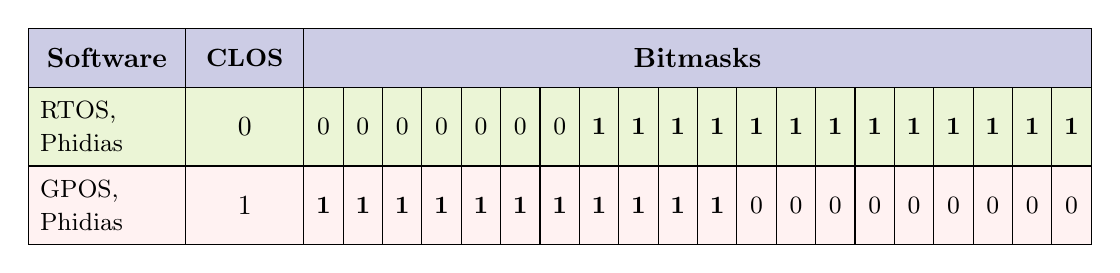
\begin{tikzpicture}

	\node at (0.5,2)[rectangle, draw=black, fill=NavyBlue!20, minimum height = 0.75cm, minimum width = 10cm, anchor=south west] (bitmasks) {\textbf{Bitmasks}};
	\node at (-1.0,2)[rectangle, draw=black, fill=NavyBlue!20, minimum height = 0.75cm, minimum width = 1.5cm, anchor=south west] (clos) {\textbf{\small{CLOS}}};
	\node at (-3.0,2)[rectangle, draw=black, fill=NavyBlue!20, minimum height = 0.75cm, minimum width = 2cm, anchor=south west] (soft) {\textbf{Software}};

	\node at (-1.0,1)[rectangle, draw=black, fill=YellowGreen!20, minimum height = 1cm, minimum width = 1.5cm, anchor=south west] (clos0) {0};
	\node at (-1.0,0)[rectangle, draw=black, fill=pink!20, minimum height = 1cm, minimum width = 1.5cm, anchor=south west] (clos1) {1};
	\node at (-3.0,1)[rectangle, draw=black, fill=YellowGreen!20, minimum height = 1cm, minimum width = 2cm, anchor=south west, text width=1.7cm]
				 (soft0) {\small{RTOS, Phidias}};
	\node at (-3.0,0)[rectangle, draw=black, fill=pink!20, minimum height = 1cm, minimum width = 2cm, anchor=south west, text width=1.7cm] 
				(soft1) {\small{GPOS, Phidias}};

	\foreach \x in {1,...,20}
		    	\node at (0.5*\x,1)[rectangle, draw=black, fill=YellowGreen!20, minimum height = 1cm, minimum width = 0.5cm, anchor=south west] (c1\x) 
							{\ifthenelse{\x>7}{\small{\textbf{1}}}{\small{0}}};

	\foreach \x in {1,...,20}
		    	\node at (0.5*\x,0)[rectangle, draw=black, fill=pink!20, minimum height = 1cm, minimum width = 0.5cm, anchor=south west] (c2\x) 
							{\ifthenelse{\x<12}{\small{\textbf{1}}}{\small{0}}};


\end{tikzpicture}
\end{center}
\ifreport
\caption{LLC Partitioning in Virtual Setup}
\fi
\label{fig-vsetup-cat-bitmasks}
\end{figure}
 
		\endgroup		
		\pause
   \item {keep some part shared for shared memory} \pause {}
   \item {repeat latency measurement experiments:}
		  \begin{itemize}
				\item {gp-guest idle}
				\item {L3 pollution from gp-guest}
		  \end{itemize}
  \end{itemize}
\end{frame}

\begin{frame}[allowframebreaks]{Cache Allocation} {Latency Reduction}
    %\begingroup
	%\tikzset{every picture/.style={scale=1}, every node/.style={scale=1}}	
	\begin{figure}[!htb]
\begin{center}
\begin{tikzpicture}  [
						my brace/.style={thick, decorate, decoration={brace, amplitude=2pt, raise=10pt,},},							
						my label/.style={below right, align=center, rotate=90, inner ysep=14pt, },
					]

		\begin{axis} [ name=plot1, height=\figheight, width=\figwidth, 
				   enlarge y limits={upper,value=0.3},  enlarge x limits=0.12,
				   ymin=0,
		           %axis y line*=left,
				   ybar=\ybarSep,  
				   x=\ybarXdist,
				   bar width=\ybarWidth,
	   			   ylabel={worst-case interrupt latency ($\mu{}s$)},
	 		       symbolic x coords={no load, cache\_pressure, forkops, fileops, threadops},
		           xtick=data,                 
		            %nodes near coords, 
					%nodes near coords align={vertical}, 
					x tick label style={rotate=0, anchor=north}, 
					xticklabel style={rotate=0,anchor=north, font=\ttfamily\small},
		            xtick align=inside,
		            xticklabel pos=left,
	   			    legend pos=north east, legend columns=-1,
				] 
		\addplot [fill=yellow!20, postaction={pattern=north east lines}, pattern color=gray] coordinates {
				(no load, 67.6)				
				(cache\_pressure, 73.7)
				(forkops, 25.9)
				(fileops, 24.7)
				(threadops, 12.4)
		      };                  

		\addplot [fill=NavyBlue!50, xshift=\xShiftLatency] coordinates {
                     (no load,141.3) 
					(cache\_pressure,132)	
					(forkops,129.9)
					(fileops,123.7)
					(threadops,146.1)
			      }
					coordinate [pos=0] (a1)
		            coordinate [pos=0.2] (a2)
		            coordinate [pos=0.4] (a3)
		            coordinate [pos=0.8] (a4)
		            coordinate [pos=1] (a5)
				  ;

		\addplot [fill=ForestGreen!60, xshift=\xShiftLatency, postaction={pattern=crosshatch dots}, pattern color=gray] coordinates {
                    (no load,120.4) 
					(cache\_pressure,112.2)	
					(forkops,108.4)
					(fileops,106.8)
					(threadops,116.9)
			      }				  	
					coordinate [pos=0] (b1)
		            coordinate [pos=0.2] (b2)
		            coordinate [pos=0.4] (b3)
		            coordinate [pos=0.8] (b4)
		            coordinate [pos=1] (b5)	
				  ;

				  \draw [my brace] (a1) -- (b1) node [my label] {\small{$+14.8\%$}};
				  \draw [my brace] (a2) -- (b2) node [my label] {\small{$+8.8\%$}};
				  \draw [my brace] (a3) -- (b3) node [my label] {\small{$+16.6\%$}};
				  \draw [my brace] (a4) -- (b4) node [my label] {\small{$+13.7\%$}};
				  \draw [my brace] (a5) -- (b5) node [my label] {\small{$+20.0\%$}};
		\legend{native, LLC shared, LLC partitioned}
		\end{axis}

		%%improvement%% 
		%% \begin{axis} [ name=plot1, height=\figheight, width=\figwidth, ybar,  enlarge y limits={upper,value=0.3},  enlarge x limits=0.12, 					
		%% 		   ymin=0, ymax=80,
		%%            axis y line*=right,
		%% 		   ybar=\ybarSep,  
		%% 		   x=\ybarXdist,
		%% 		   bar width=\ybarWidth,
	   	%% 		   ylabel={improvement \%},
	 	%% 	       symbolic x coords={no load, cache pressure, forkops, fileops, threadops},
		%%            xtick=data,                 
		%%             nodes near coords, 
		%% 			nodes near coords align={vertical}, 
		%% 			x tick label style={rotate=0, anchor=north}, 
		%% 			xticklabel style={rotate=0,anchor=north},
		%%             xtick align=inside,
		%%             xticklabel pos=left,
	   	%% 		    legend pos=north east, legend columns=-1,
		%%          ]  
		%% \addplot [fill=OliveGreen!50, xshift=\xShiftImprove, postaction={pattern=crosshatch dots}] coordinates {
        %%             (no load, 14.8) 
		%% 			(cache pressure,8.8)	
		%% 			(forkops,16.6)
		%% 			(fileops,13.7)
		%% 			(threadops,20)
		%% 	      };
		%% \legend{improvement}
		%% \end{axis}

%%%%%%%%%%%%%%%%%%for defense presentation%%%%%%%%%%%%%%%%%%%%
\ifdefense

\end{tikzpicture}
\end{center}
\label{plot-cat1}
\end{figure}
	
\begin{figure}[!htb]
\begin{center}
\begin{tikzpicture}  [
						my brace/.style={thick, decorate, decoration={brace, amplitude=2pt, raise=10pt,},},							
						my label/.style={below right, align=center, rotate=90, inner ysep=14pt, },
					]

\fi
%%%%%%%%%%%%%%%%%%%%%ENDIF%%%%%%%%%%%%%%%%%%%%%%%%%%%%%%%%%
	\begin{axis} [ name=plot2, \atCmdLowerPlot, 
					height=\figheight, width=\figwidth, enlarge y limits={upper,value=0.3},  
					enlarge x limits=0.12,
				   ymin=0,
		           %axis y line*=left,
				   ybar=\ybarSep,
				   x=\ybarXdist,
				   bar width=\ybarWidth,
	   			   ylabel={average-case interrupt latency ($\mu{}s$)},
	 		       symbolic x coords={no load, cache\_pressure, forkops, fileops, threadops},
		           xtick=data,                 
		            %nodes near coords, 
					%nodes near coords align={vertical}, 
					x tick label style={rotate=0, anchor=north, font=\ttfamily\small}, 
					xticklabel style={rotate=0,anchor=north},
		            xtick align=inside,
		            xticklabel pos=left,
	   			    legend pos=north east, legend columns=-1,
				 ] 
		\addplot [fill=yellow!20, postaction={pattern=north east lines}, pattern color=gray] coordinates {
				(no load, 44.2)				
				(cache\_pressure, 43.1)
				(forkops, 6.1)
				(fileops, 6.1)
				(threadops, 5)
			   };  
                   
		\addplot [fill=NavyBlue!50, xshift=\xShiftLatency] coordinates {
                    (no load,19.1) 
					(cache\_pressure,28.5)	
					(forkops,13.1)
					(fileops,13.8)
					(threadops,19.6)			
			      }
					coordinate [pos=0] (a1)
		            coordinate [pos=0.2] (a2)
		            coordinate [pos=0.4] (a3)
		            coordinate [pos=0.8] (a4)
		            coordinate [pos=1] (a5)
				  ;
		\addplot [fill=ForestGreen!60, xshift=\xShiftLatency, postaction={pattern=crosshatch dots}, pattern color=gray] coordinates {
                     (no load,15.7) 
					(cache\_pressure,15.2)	
					(forkops,9.9)
					(fileops,10)
					(threadops,12.4)			
			      }				  	
					coordinate [pos=0] (b1)
		            coordinate [pos=0.2] (b2)
		            coordinate [pos=0.4] (b3)
		            coordinate [pos=0.8] (b4)
		            coordinate [pos=1] (b5)	
				  ;

				  \draw [my brace] (a1) -- (b1) node [my label] {\small{$+17.8\%$}};
				  \draw [my brace] (a2) -- (b2) node [my label] {\small{$+46.6\%$}};
				  \draw [my brace] (a3) -- (b3) node [my label] {\small{$+24.4\%$}};
				  \draw [my brace] (a4) -- (b4) node [my label] {\small{$+27.5\%$}};
				  \draw [my brace] (a5) -- (b5) node [my label] {\small{$+36.7\%$}};
	\legend{native, LLC shared, LLC partitioned}
	\end{axis}

	%%improvement%%
	%% \begin{axis} [ name=plot2, \atCmdLowerPlot,  height=\figheight, width=\figwidth, ybar,  
	%% 				enlarge y limits={upper,value=0.3},  enlarge x limits=0.12, ymin=0, ymax=80,
	%% 	           axis y line*=right,
	%% 			   ybar=\ybarSep,  
	%% 			   x=\ybarXdist,             
	%% 			   bar width=\ybarWidth,
	%%    			   ylabel={improvement \%},
	%%  		       symbolic x coords={no load, cache pressure, forkops, fileops, threadops},
	%% 	           xtick=data,                 
	%% 	            nodes near coords, 
	%% 				nodes near coords align={vertical}, 
	%% 				x tick label style={rotate=0, anchor=north}, 
	%% 				xticklabel style={rotate=0,anchor=north},
	%% 	            xtick align=inside,
	%% 	            xticklabel pos=left,
	%%    			    legend pos=north east, legend columns=-1,
	%% 	         ]  
	%% \addplot [fill=OliveGreen!50, xshift=\xShiftImprove, postaction={pattern=crosshatch dots}] coordinates {
    %%                 (no load,17.8) 
	%% 				(cache pressure,46.6)	
	%% 				(forkops,24.4)
	%% 				(fileops,27.5)
	%% 				(threadops,36.7)
	%% 		      };
	%% \legend{improvement}
	%% \end{axis}

\end{tikzpicture}
\end{center}
\ifreport
\caption{Interrupt latency comparison of shared LLC and partitioned LLC}
\label{plot-cat}
\else
\label{plot-cat2}
\fi
\end{figure}


	%\endgroup
\end{frame}

%%%%%%%%%%%%%%%%%~~~SUB SECTION~~~%%%%%%%%%%%%%%%%%
\subsection{TLB Partitioning using VPIDs}
\begin{frame}{TLB Partitioning using VPIDs} {Methodology}
   \begin{itemize}
     \item {extend Phidias to support VPIDs} \pause {}
     \item {use VPIDs to isolate Phidias TLB cache from rt-guest} \pause {}
  	 \item {repeat latency measurement experiments}
  \end{itemize}
\end{frame}

\begin{frame}[allowframebreaks]{TLB Partitioning using VPIDs} {Latency Reduction}
    %\begingroup
	%\tikzset{every picture/.style={scale=0.8}, every node/.style={scale=0.8}}	
	\begin{figure}[!htb]
\begin{center}
\begin{tikzpicture}  [
						my brace/.style={thick, decorate, decoration={brace, amplitude=3pt, raise=4pt,},},							
						my label/.style={below right, align=center, rotate=90, inner ysep=10pt, },
						another label/.style={below right, align=center, rotate=90, inner ysep=5pt, },
					]

	\begin{axis} [ name=plot1, height=\figheight, width=\figwidth, 
				   enlarge y limits={upper,value=0.3},  enlarge x limits=0.12,
				   ymin=0,
		           %axis y line*=left,
				   ybar=\ybarSep,  
				   x=\ybarXdist,
				   bar width=\ybarWidth,
	   			   ylabel={worst-case  latency ($\mu{}s$)},
	 		       symbolic x coords={no load, cache\_pressure, forkops, fileops, threadops},
		           xtick=data,                 
		            %nodes near coords, 
					%nodes near coords align={vertical}, 
					x tick label style={rotate=0, anchor=north, font=\ttfamily\small}, 
					xticklabel style={rotate=0,anchor=north},
		            xtick align=inside,
		            xticklabel pos=left,
	   			    legend pos=north east, legend columns=-1,
				 ]                    
	\addplot [fill=NavyBlue!50, xshift=\xShiftLatency] coordinates {
                    (no load,129.5) 
					(cache\_pressure,145.6)	
					(forkops,128.2)
					(fileops,127.1)
					(threadops,169.6)
			      }
					coordinate [pos=0] (a1)
		            coordinate [pos=0.2] (a2)
		            coordinate [pos=0.4] (a3)
		            coordinate [pos=0.8] (a4)
		            coordinate [pos=1] (a5)
				  ;

	\addplot [fill=ForestGreen!60, xshift=\xShiftLatency, postaction={pattern=crosshatch dots}, pattern color=gray] coordinates {
                    (no load,130.5) 
					(cache\_pressure,131.7)	
					(forkops,124.8)
					(fileops,123.7)
					(threadops,148.8)
			      }
				  	coordinate [pos=0] (b1)
		            coordinate [pos=0.2] (b2)
		            coordinate [pos=0.4] (b3)
		            coordinate [pos=0.8] (b4)
		            coordinate [pos=1] (b5)	
				  ;

				  \draw [thick, |-|] ([xshift=4pt]a1) -- ([xshift=4pt]b1) node [another label] {\small{$-0.8\%$}};
				  \draw [thick, |-|] ([xshift=4pt]a2) -- ([xshift=4pt]b2) node [another label] {\small{$+9.5\%$}};
				  \draw [thick, |-|] ([xshift=4pt]a3) -- ([xshift=4pt]b3) node [another label] {\small{$+2.6\%$}};
				  \draw [thick, |-|] ([xshift=4pt]a4) -- ([xshift=4pt]b4) node [another label] {\small{$+2.7\%$}};
				  \draw [my brace] (a5) -- (b5) node [my label] {\small{$+12.2\%$}};
	\legend{shared TLB, isolated TLB}
	\end{axis}

	%%improvement%%
	%% \begin{axis} [ name=plot1, height=\figheight, width=\figwidth, ybar,  enlarge y limits={upper,value=0.3},  enlarge x limits=0.12, 					
	%% 			   ymin=0, ymax=80,
	%% 	           axis y line*=right,
	%% 			   ybar=\ybarSep,  
	%% 			   x=\ybarXdist,
	%% 			   bar width=\ybarWidth,
	%%    			   ylabel={improvement \%},
	%%  		       symbolic x coords={no load, cache pressure, forkops, fileops, threadops},
	%% 	           xtick=data,                 
	%% 	            nodes near coords, 
	%% 				nodes near coords align={vertical}, 
	%% 				x tick label style={rotate=0, anchor=north}, 
	%% 				xticklabel style={rotate=0,anchor=north},
	%% 	            xtick align=inside,
	%% 	            xticklabel pos=left,
	%%    			    legend pos=north east, legend columns=-1,
	%% 	         ]  
	%% 	\addplot [fill=OliveGreen!50, xshift=\xShiftImprove, postaction={pattern=crosshatch dots}] coordinates {
    %%                 (no load, 0) 
	%% 				(cache pressure,9.5)	
	%% 				(forkops,2.6)
	%% 				(fileops,2.7)
	%% 				(threadops,12.2)
	%% 		      };
	%% 	\legend{improvement}
	%% 	\end{axis}
%%%%%%%%%%%%%%%%%%for defense presentation%%%%%%%%%%%%%%%%%%%%
\ifdefense

\end{tikzpicture}
\end{center}
\label{plot-vpid1}
\end{figure}
	
\begin{figure}[!htb]
\begin{center}
\begin{tikzpicture} [
						my brace/.style={thick, decorate, decoration={brace, amplitude=3pt, raise=4pt,},},							
						my label/.style={below right, align=center, rotate=90, inner ysep=10pt, },
					]

\fi
%%%%%%%%%%%%%%%%%%%%%ENDIF%%%%%%%%%%%%%%%%%%%%%%%%%%%%%%%%%

		\begin{axis} [	 name=plot2, \atCmdLowerPlot, 
					height=\figheight, width=\figwidth, enlarge y limits={upper,value=0.3},  
					enlarge x limits=0.12,
				   ymin=10,
		           %axis y line*=left,
				   ybar=\ybarSep,
				   x=\ybarXdist,
				   bar width=\ybarWidth,
	   			   ylabel={average-case latency ($\mu{}s$)},
	 		       symbolic x coords={no load, cache\_pressure, forkops, fileops, threadops},
		           xtick=data,                 
		            %nodes near coords, 
					%nodes near coords align={vertical}, 
					x tick label style={rotate=0, anchor=north}, 
					xticklabel style={rotate=0,anchor=north, font=\ttfamily\small},
		            xtick align=inside,
		            xticklabel pos=left,
	   			    legend pos=north east, legend columns=-1,
					]                    
		\addplot [fill=NavyBlue!50, xshift=\xShiftLatency] coordinates {
                    (no load,18.2) 
					(cache\_pressure,18.1)	
					(forkops,12.6)
					(fileops,14.5)
					(threadops,17)			
			      }
					coordinate [pos=0] (a1)
		            coordinate [pos=0.2] (a2)
		            coordinate [pos=0.4] (a3)
		            coordinate [pos=0.8] (a4)
		            coordinate [pos=1] (a5)
				  ;
		\addplot [fill=ForestGreen!60, xshift=\xShiftLatency, postaction={pattern=crosshatch dots}, pattern color=gray] coordinates {
                    (no load,17) 
					(cache\_pressure,16.7)	
					(forkops,11.6)
					(fileops,13.4)
					(threadops,15.4)			
			      }
				  	coordinate [pos=0] (b1)
		            coordinate [pos=0.2] (b2)
		            coordinate [pos=0.4] (b3)
		            coordinate [pos=0.8] (b4)
		            coordinate [pos=1] (b5)	
				  ;

				  \draw [my brace] (a1) -- (b1) node [my label] {\small{$+6.5\%$}};
				  \draw [my brace] (a2) -- (b2) node [my label] {\small{$+7.7\%$}};
				  \draw [my brace] (a3) -- (b3) node [my label] {\small{$+7.9\%$}};
				  \draw [my brace] (a4) -- (b4) node [my label] {\small{$+7.5\%$}};
				  \draw [my brace] (a5) -- (b5) node [my label] {\small{$+9.4\%$}};
		\legend{shared TLB, isolated TLB}
		\end{axis}

	%%improvement%%
	%% \begin{axis} [ name=plot2, \atCmdLowerPlot,  height=\figheight, width=\figwidth, ybar,  
	%% 				enlarge y limits={upper,value=0.3},  enlarge x limits=0.12, ymin=0, ymax=80,
	%% 	           axis y line*=right,
	%% 			   ybar=\ybarSep,  
	%% 			   x=\ybarXdist,             
	%% 			   bar width=\ybarWidth,
	%%    			   ylabel={improvement \%},
	%%  		       symbolic x coords={no load, cache pressure, forkops, fileops, threadops},
	%% 	           xtick=data,                 
	%% 	            nodes near coords, 
	%% 				nodes near coords align={vertical}, 
	%% 				x tick label style={rotate=0, anchor=north}, 
	%% 				xticklabel style={rotate=0,anchor=north},
	%% 	            xtick align=inside,
	%% 	            xticklabel pos=left,
	%%    			    legend pos=north east, legend columns=-1,
	%% 	         ]  
	%% \addplot [fill=OliveGreen!50, xshift=\xShiftImprove, postaction={pattern=crosshatch dots}] coordinates {
    %%                 (no load,6.5)
	%% 				(cache pressure,7.7)	
	%% 				(forkops,7.9)
	%% 				(fileops,7.5)
	%% 				(threadops,9.4)
	%% 		      };
	%% \legend{improvement}
	%% \end{axis}

\end{tikzpicture}
\end{center}
\ifreport
\caption{Interrupt latency comparison of shared and isolated TLB between guest and Phidias}
\label{plot-vpid}
\else
\label{plot-vpid2}
\fi
\end{figure}


	%\endgroup
\end{frame}

%%%%%%%%%%%%%%%%%~~~SUB SECTION~~~%%%%%%%%%%%%%%%%%
\subsection{CAT, DII, and VPID Combined}
\begin{frame}[allowframebreaks]{CAT, DII, and VPID Combined} {Latency Reduction}
    %\begingroup
	%\tikzset{every picture/.style={scale=0.8}, every node/.style={scale=0.8}}	
	\begin{figure}[!htb]
\begin{center}
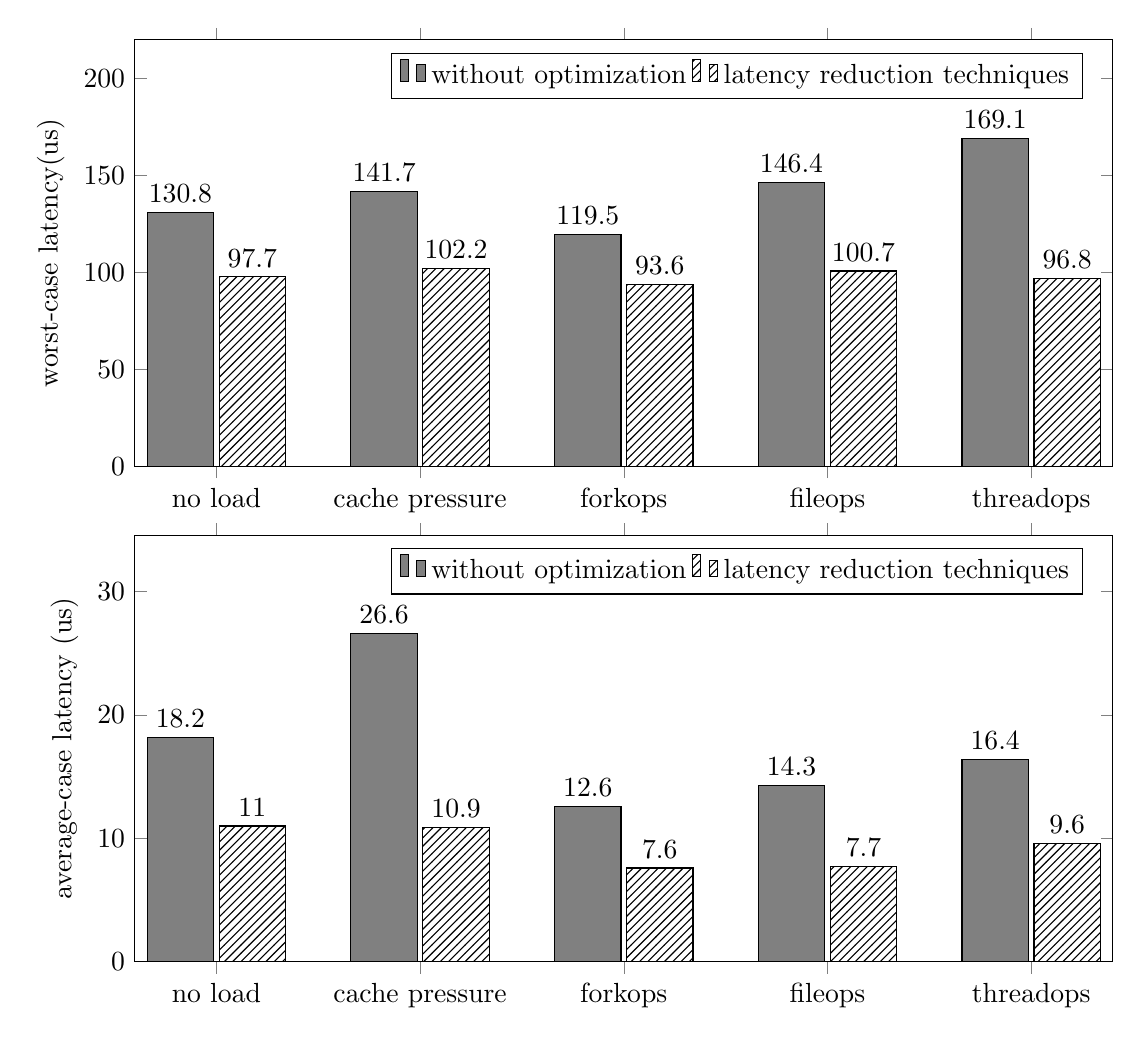
\begin{tikzpicture} %[scale = 1.2]

\begin{axis} [name=plot1, height=7cm, width=14cm, ybar=2pt, enlarge y limits={upper,value=0.3},  %enlargelimits=0.3, 
			ymin=0,
			legend pos=north east, legend columns=-1,
                       %legend style={at={(0.5,-0.1)}, anchor=north, legend columns=-1}, 
                       ylabel={worst-case latency(us)}, %title=no pollution from gp-guest, 
		       bar width= 24pt,
			%symbolic x coords={without VPID, with VPID},
                       symbolic x coords={no load, cache pressure, forkops, fileops, threadops},
                       xtick=data, nodes near coords, nodes near coords align={vertical}, x tick label style={rotate=0,anchor=north}, ]                    
	\addplot [fill=black!50] coordinates {
                    (no load,130.8) 
					(cache pressure,141.7)	
					(forkops,119.5)
					(fileops,146.4)
					(threadops,169.1)
			      };

	\addplot [postaction={pattern=north east lines}] coordinates {
                    (no load,97.7) 
					(cache pressure,102.2)	
					(forkops,93.6)
					(fileops,100.7)
					(threadops,96.8)
			      };
\legend{without optimization, latency reduction techniques}
\end{axis}


\begin{axis} [name=plot2, at={($(plot1.west)+(0,-9cm)$)}, height=7cm,  width=14cm, ybar=2pt, enlarge y limits={upper,value=0.3},  %enlargelimits=0.3, 
			ymin=0,
                       legend pos=north east, legend columns=-1,
			%legend style={at={(0.5,-0.1)}, anchor=north, legend columns=-1}, 
                       ylabel={average-case latency (us)}, %title=no pollution from gp-guest, 
		       bar width= 24pt,
                       %symbolic x coords={without VPID, with VPID},
			symbolic x coords={no load, cache pressure, forkops, fileops, threadops},
                       xtick=data, nodes near coords, nodes near coords align={vertical}, x tick label style={rotate=0,anchor=north}, ]                    
	\addplot [fill=black!50] coordinates {
                    (no load,18.2) 
					(cache pressure,26.6)	
					(forkops,12.6)
					(fileops,14.3)
					(threadops,16.4)			
			      };
	\addplot [postaction={pattern=north east lines}] 				
				coordinates {
                    (no load,11) 
					(cache pressure,10.9)	
					(forkops,7.6)
					(fileops,7.7)
					(threadops,9.6)			
			      };
\legend{without optimization, latency reduction techniques}
\end{axis}

\end{tikzpicture}

%\begin{tabular}{c c c c c}
%\multicolumn{5}{c}{Percentage Improvement}
%no load & cache pressure & forkops & fileops & threadops \\
%25.3 & 27.9 & 21.7 & 31.2 & 42.8 \\
%\end{tabular}

\end{center}
\ifreport
\caption{Comparison of interrupt latency when no optimization is deployed versus latency reduction techniques (direct interrupt, cache allocation, isolated TLB cache)}
\fi
\label{plot-allopt}
\end{figure}


	%\endgroup
\end{frame}

%%%%%%%%%%%%%%%%%~~~...SECTION...~~~%%%%%%%%%%%%%%%%%
\section{Conclusion}
\subsection{Concluding Remarks}
\begin{frame}{Concluding Remarks}
  \begin{itemize}
  \item {virtualization overhead increased latency twice {from $80\mu{}s$ to $170\mu{}s$}} \pause{}
  \item {CAT, DII and VPID reduced virtualization overhead}  \pause{}
		\begin{itemize}
			\item{worst-case more than $21$\%}  \pause{}
			\item{average-case more than $39$\%}  \pause{}
		\end{itemize}
  \item {virtual setup can meet real-time constraints in the order of $90\mu{}s-110\mu{}s$} \pause{}
	  	\begin{itemize}
	     	\item {which is not far from native setup  $20\mu{}s-80\mu{}s$}
		\end{itemize}
  \end{itemize}
\end{frame}
\subsection{Future Work}
\begin{frame}{Future Work}
  \begin{itemize}
	\item {resource contention: L1/L2 partitioning} \pause{}
	\item {processor with smaller caches} \pause{}
    \item {reduce guest traps:} 
		  \begin{itemize}
			\item {MSR writes} \pause{}
			\item {IO access}
		  \end{itemize}
  \end{itemize}
\end{frame}

\begin{frame}
  \center\LARGE{Thank you!}
\end{frame}

\begin{frame}[allowframebreaks]{Virtualization Overhead} {Cumulative Distribution Function (CDF)}
  	%\begingroup
	%\tikzset{every picture/.style={scale=0.8}, every node/.style={scale=0.8}}	
	\begin{figure}[!htb]
\begin{center}

\begin{tikzpicture}


\begin{axis}[name=plot1, height=6cm, width=12cm, ymin=0, ymax=1, xmin=0, 		
		xlabel=latency(us), 
		ylabel=probability,
		title style={yshift=-2ex},
		legend pos=south east,
		title=load:cache pressure,
		]
	\addplot [thick, blue] table[x=Latency,y=Probability] {./figures/native_cachepressure_10k_cdf.dat};
	\addplot [thick, red] table[x=Latency,y=Probability] {./figures/virt_cachepressure_10k_cdf.dat};
	\legend {\small{native (max 77.9)}, \small{virtual (max 131.1)}}
\end{axis}


\begin{axis}[name=plot2, at={($(plot1.south west)+(0,-6.5cm)$)}, height=6cm, width=12cm, ymin=0, ymax=1, xmin=0, 
		legend pos=south east,
		xlabel=latency(us), 
		ylabel=probability, 
		title style={yshift=-2ex},
		title=load:threadops,
		]
	\addplot [thick, blue] table[x=Latency,y=Probability] {./figures/native_threadops_cdf.dat};	
	\addplot [thick, red] table[x=Latency,y=Probability] {./figures/virt_threadops_10k_cdf.dat};
	\legend {\small{native (max 12.4)}, \small{virtual (max 169.1)}}
\end{axis}



\begin{axis}[name=plot3, at={($(plot2.south west)+(0,-6.5cm)$)}, height=6cm, width=12cm, ymin=0, ymax=1, xmin=0, 
		legend pos=south east,
		xlabel=latency(us), 
		ylabel=probability, 
		title style={yshift=-2ex},
		title=load:forkops,
		]
	\addplot [thick, blue] table[x=Latency,y=Probability] {./figures/native_forkops_10k_cdf.dat};	
	\addplot [thick, red] table[x=Latency,y=Probability] {./figures/virt_forkops2_10k_cdf.dat};
	\legend {\small{native (max 25.9)}, \small{virtual (max 119.5)}}
\end{axis}

\end{tikzpicture}
\end{center}
\caption{Comparison of interrupt latency CDF between native and virtual setup for different load conditions}
\label{plot-cdf-native-vs-virtual}
\end{figure}

	%\endgroup
\end{frame}

\begin{frame}[allowframebreaks]{Overhead Components} {Context-Switch time CDF}
    \begingroup
	\tikzset{every picture/.style={scale=0.9}, every node/.style={scale=0.9}}	
	\begin{figure}[!htb]
\begin{center}

\begin{tikzpicture}


\begin{axis}[name=plot1, height=8cm, width=12cm,
		legend pos=south east,
		xlabel=context-switch overhead ($\mu{}s$), 
		ylabel=Probability, enlargelimits=0.05,
		%ymajorgrids=true, grid style = very thin,
		]
	\addplot [ultra thick, blue] table[x=Latency,y=Probability] {./figures/vmexitentry_10k_cdf.dat};
	\addplot [very thick, red, dashed] table[x=Latency,y=Probability] {./figures/vmexitentry_cachepressure_10k_cdf.dat};
	\legend {\small{no load (max 17.2)}, \small{cache pressure (max 86.8)}}
\end{axis}

\end{tikzpicture}
\end{center}
\ifreport
\caption{CDF of context-switch overhead}
\fi
\label{plot-cdf-contextswitch}
\end{figure}

	\endgroup
\end{frame}

\begin{frame}{VT-x Properties and Real-Time Guests} {non-deterministic behavior}
   \begin{itemize}
    \item {big multi-level caches} \pause{}
    \item {big data structures to manage VMs} \pause{}
    \item {unknown instruction behavior (e.g. INVVPID)}
   \end{itemize}
\end{frame}

\begin{frame}[allowframebreaks]{CAT, DII, and VPID Combined} {CDF}
    %\begingroup
	%\tikzset{every picture/.style={scale=0.8}, every node/.style={scale=0.8}}	
	\begin{figure}[!htb]
\begin{center}

\begin{tikzpicture}


\begin{axis}[name=plot1, height=6cm, width=12cm, ymin=0, ymax=1, xmin=0, 		
		xlabel=latency(us), 
		ylabel=probability,
		title style={yshift=-2ex},
		legend pos=south east,
		title=load:cache pressure,
		]
	\addplot [thick, blue] table[x=Latency,y=Probability] {./figures/native_cachepressure_10k_cdf.dat};
	\addplot [thick, red] table[x=Latency,y=Probability] {./figures/virt_cachepressure_10k_cdf.dat};
	\addplot [very thick, green] table[x=Latency,y=Probability] {./figures/allopt_cachepressure_10k_cdf.dat};
	\legend {\small{native (avg 44.2, max 77.9)}, \small{virtual (avg 18.2, max 131.1)}, \small{optimized (avg 11, max 100.4)}}
\end{axis}


\begin{axis}[name=plot2, at={($(plot1.south west)+(0,-6.5cm)$)}, height=6cm, width=12cm, ymin=0, ymax=1, xmin=0, 
		legend pos=south east,
		xlabel=latency(us), 
		ylabel=probability, 
		title style={yshift=-2ex},
		title=load:threadops,
		]
	\addplot [thick, blue] table[x=Latency,y=Probability] {./figures/native_threadops_cdf.dat};	
	\addplot [thick, red] table[x=Latency,y=Probability] {./figures/virt_threadops_10k_cdf.dat};
	\addplot [very thick, green] table[x=Latency,y=Probability] {./figures/allopt_threadops_10k_cdf.dat};
	\legend {\small{native (avg 5, max 12.4)}, \small{virtual (avg 16.4, max 169.1)}, \small{optimized (avg 9.6, max 96.8)}}
\end{axis}



\begin{axis}[name=plot3, at={($(plot2.south west)+(0,-6.5cm)$)}, height=6cm, width=12cm, ymin=0, ymax=1, xmin=0, 
		legend pos=south east,
		xlabel=latency(us), 
		ylabel=probability, 
		title style={yshift=-2ex},
		title=load:forkops,
		]
	\addplot [thick, blue] table[x=Latency,y=Probability] {./figures/native_forkops_10k_cdf.dat};	
	\addplot [thick, red] table[x=Latency,y=Probability] {./figures/virt_forkops2_10k_cdf.dat};
	\addplot [very thick, green] table[x=Latency,y=Probability] {./figures/allopt_forkops_10k_cdf.dat};
	\legend {\small{native (avg 6.1, max 25.9)}, \small{virtual (avg 12.6, max 119.5)}, \small{optimized (avg 7.6, max 97.7)}}
\end{axis}

\end{tikzpicture}
\end{center}
\ifreport
\caption{Comparison of interrupt latency CDF between native and virtual setup for different load conditions}
\fi
\label{plot-cdf-native-virtual-optimiz}
\end{figure}

	%\endgroup
\end{frame}

\end{document}


